%%%%%%%%%%%%%%%%%%%%%%%%%%%%%%%%%%%%%%%%%%%%%%%%%%%%%%%%%%%%%%%%%%%%%%%%%%%%%%%%
%%%%%%%%%%%%%%%%%%%%%%%%%%%%%%%%%%%%%%%%%%%%%%%%%%%%%%%%%%%%%%%%%%%%%%%%%%%%%%%%
%%                                                                            %%
%% thesistemplate.tex version 3.20 (2018/08/31)                               %%
%% The LaTeX template file to be used with the aaltothesis.sty (version 3.20) %%
%% style file.                                                                %%
%% This package requires pdfx.sty v. 1.5.84 (2017/05/18) or newer.            %%
%%                                                                            %%
%% This is licensed under the terms of the MIT license below.                 %%
%%                                                                            %%
%% Written by Luis R.J. Costa.                                                %%
%% Currently developed at the Learning Services of Aalto University School of %%
%% Electrical Engineering by Luis R.J. Costa since May 2017.                  %%
%%                                                                            %%
%% Copyright 2017-2018, by Luis R.J. Costa, luis.costa@aalto.fi,              %%
%% Copyright 2017-2018 Swedish translations in aaltothesis.cls by Elisabeth   %%
%% Nyberg, elisabeth.nyberg@aalto.fi and Henrik Wallén,                       %%
%% henrik.wallen@aalto.fi.                                                    %%
%% Copyright 2017-2018 Finnish documentation in the template opinnatepohja.tex%%
%% by Perttu Puska, perttu.puska@aalto.fi, and Luis R.J. Costa.               %%
%% Copyright 2018 English template thesistemplate.tex by Luis R.J. Costa.     %%
%% Copyright 2018 Swedish template kandidatarbetsbotten.tex by Henrik Wallen. %%
%%                                                                            %%
%% Permission is hereby granted, free of charge, to any person obtaining a    %%
%% copy of this software and associated documentation files (the "Software"), %%
%% to deal in the Software without restriction, including without limitation  %%
%% the rights to use, copy, modify, merge, publish, distribute, sublicense,   %%
%% and/or sell copies of the Software, and to permit persons to whom the      %%
%% Software is furnished to do so, subject to the following conditions:       %%
%% The above copyright notice and this permission notice shall be included in %%
%% all copies or substantial portions of the Software.                        %%
%% THE SOFTWARE IS PROVIDED "AS IS", WITHOUT WARRANTY OF ANY KIND, EXPRESS OR %%
%% IMPLIED, INCLUDING BUT NOT LIMITED TO THE WARRANTIES OF MERCHANTABILITY,   %%
%% FITNESS FOR A PARTICULAR PURPOSE AND NONINFRINGEMENT. IN NO EVENT SHALL    %%
%% THE AUTHORS OR COPYRIGHT HOLDERS BE LIABLE FOR ANY CLAIM, DAMAGES OR OTHER %%
%% LIABILITY, WHETHER IN AN ACTION OF CONTRACT, TORT OR OTHERWISE, ARISING    %%
%% FROM, OUT OF OR IN CONNECTION WITH THE SOFTWARE OR THE USE OR OTHER        %%
%% DEALINGS IN THE SOFTWARE.                                                  %%
%%                                                                            %%
%%                                                                            %%
%%%%%%%%%%%%%%%%%%%%%%%%%%%%%%%%%%%%%%%%%%%%%%%%%%%%%%%%%%%%%%%%%%%%%%%%%%%%%%%%
%%                                                                            %%
%%                                                                            %%
%% An example for writting your thesis using LaTeX                            %%
%% Original version and development work by Luis Costa, changes to the text   %% 
%% in the Finnish template by Perttu Puska.                                   %%
%% Support for Swedish added 15092014                                         %%
%% PDF/A-b support added on 15092017                                          %%
%% PDF/A-2 support added on 24042018                                          %%
%%                                                                            %%
%% This example consists of the files                                         %%
%%         thesistemplate.tex (version 3.20) (for text in English)            %%
%%         opinnaytepohja.tex (version 3.20) (for text in Finnish)            %%
%%         kandidatarbetsbotten.tex (version 1.00) (for text in Swedish)      %%
%%         aaltothesis.cls (versio 3.20)                                      %%
%%         kuva1.eps (graphics file)                                          %%
%%         kuva2.eps (graphics file)                                          %%
%%         kuva1.jpg (graphics file)                                          %%
%%         kuva2.jpg (graphics file)                                          %%
%%         kuva1.png (graphics file)                                          %%
%%         kuva2.png (graphics file)                                          %%
%%         kuva1.pdf (graphics file)                                          %%
%%         kuva2.pdf (graphics file)                                          %%
%%                                                                            %%
%%                                                                            %%
%% Typeset in Linux either with                                               %%
%% pdflatex: (recommended method)                                             %%
%%             $ pdflatex thesistemplate                                      %%
%%             $ pdflatex thesistemplate                                      %%
%%                                                                            %%
%%   The result is the file thesistemplate.pdf that is PDF/A compliant, if    %%
%%   you have chosen the proper \documenclass options (see comments below)    %%
%%   and your included graphics files have no problems.
%%                                                                            %%
%% Or                                                                         %%
%% latex: (this method is not recommended)                                    %%
%%             $ latex thesistemplate                                         %%
%%             $ latex thesistemplate                                         %%
%%                                                                            %%
%%   The result is the file thesistemplate.dvi, which is converted to ps      %%
%%   format as follows:                                                       %%
%%                                                                            %%
%%             $ dvips thesistemplate -o                                      %%
%%                                                                            %%
%%   and then to pdf as follows:                                              %%
%%                                                                            %%
%%             $ ps2pdf thesistemplate.ps                                     %%
%%                                                                            %%
%%   This pdf file is not PDF/A compliant. You must must make it so using,    %%
%%   e.g., Acrobat Pro or PDF-XChange.                                        %%
%%                                                                            %%
%%                                                                            %%
%% Explanatory comments in this example begin with the characters %%, and     %%
%% changes that the user can make with the character %                        %%
%%                                                                            %%
%%%%%%%%%%%%%%%%%%%%%%%%%%%%%%%%%%%%%%%%%%%%%%%%%%%%%%%%%%%%%%%%%%%%%%%%%%%%%%%%
%%%%%%%%%%%%%%%%%%%%%%%%%%%%%%%%%%%%%%%%%%%%%%%%%%%%%%%%%%%%%%%%%%%%%%%%%%%%%%%%
%%
%% WHAT is PDF/A
%%
%% PDF/A is the ISO-standardized version of the pdf. The standard's goal is to
%% ensure that he file is reproducable even after a long time. PDF/A differs
%% from pdf in that it allows only those pdf features that support long-term
%% archiving of a file. For example, PDF/A requires that all used fonts are
%% embedded in the file, whereas a normal pdf can contain only a link to the
%% fonts in the system of the reader of the file. PDF/A also requires, among
%% other things, data on colour definition and the encryption used.
%% Currently three PDF/A standards exist:
%% PDF/A-1: based on PDF 1.4, standard ISO19005-1, published in 2005.
%%          Includes all the requirements essential for long-term archiving.
%% PDF/A-2: based on PDF 1.7, standard ISO19005-2, published in 2011.
%%          In addition to the above, it supports embedding of OpenType fonts,
%%          transparency in the colour definition and digital signatures.
%% PDF/A-3: based on PDF 1.7, standard ISO19005-3, published in 2012.
%%          Differs from the above only in that it allows embedding of files in
%%          any format (e.g., xml, csv, cad, spreadsheet or wordprocessing
%%          formats) into the pdf file.
%% PDF/A-1 files are not necessarily PDF/A-2 -compatible and PDF/A-2 are not
%% necessarily PDF/A-1 -compatible.
%% All of the above PDF/A standards have two levels:
%% b: (basic) requires that the visual appearance of the document is reliably
%%    reproduceable.
%% a (accessible) in addition to the b-level requirements, specifies how
%%   accessible the pdf file is to assistive software, say, for the physically
%%   impaired.
%% For more details on PDF/A, see, e.g., https://en.wikipedia.org/wiki/PDF/A
%%
%%
%% WHICH PDF/A standard should my thesis conform to?
%%
%% Primarily to the PDF/A-1b standard. All the figures and graphs typically
%% use in thesis work do not require transparency features, a basic '2-D'
%% visualisation suffices. The font to be used are specified in this template
%% and they should not be changed. However, if you have figures where
%% transparency characteristics matter, use the PDF/A-2b standard. Do not use
%% the PDF/A-3b standard for your thesis.
%%
%%
%% WHAT graphics format can I use to produce my PDF/A compliant file?
%%
%% When using pdflatex to compile your work, use jpg, png or pdf files. You may
%% have PDF/A compliance problems with figures in pdf format. Do not use PDF/A
%% compliant graphics files.
%% If you decide to use latex to compile your work, the only acceptable file
%% format for your figure is eps. DO NOT use the ps format for your figures.

%% USE one of these:
%% * the first when using pdflatex, which directly typesets your document in the
%%   chosen pdf/a format and you want to publish your thesis online,

%% * the second when you want to print your thesis to bind it, or
%% * the third when producing a ps file and a pdf/a from it.
%%
\documentclass[english, 12pt, a4paper, elec, utf8, a-1b, online]{aaltothesis}
%\documentclass[english, 12pt, a4paper, elec, utf8, a-1b]{aaltothesis}
%\documentclass[english, 12pt, a4paper, elec, dvips, online]{aaltothesis}

%% Use the following options in the \documentclass macro above:
%% your school: arts, biz, chem, elec, eng, sci
%% the character encoding scheme used by your editor: utf8, latin1
%% thesis language: english, finnish, swedish
%% make an archiveable PDF/A-1b or PDF/A-2b compliant file: a-1b, a-2b
%%                    (with pdflatex, a normal pdf containing metadata is
%%                     produced without the a-*b option)
%% typeset in symmetric layout and blue hypertext for online publication: online
%%            (no option is the default, resulting in a wide margin on the
%%             binding side of the page and black hypertext)
%% two-sided printing: twoside (default is one-sided printing)
%%

%% Use one of these if you write in Finnish (see the Finnish template
%% opinnaytepohja.tex)
%\documentclass[finnish, 12pt, a4paper, elec, utf8, a-1b, online]{aaltothesis}
%\documentclass[finnish, 12pt, a4paper, elec, utf8, a-1b]{aaltothesis}
%\documentclass[finnish, 12pt, a4paper, elec, dvips, online]{aaltothesis}

\usepackage{graphicx}

%% Math fonts, symbols, and formatting; these are usually needed
\usepackage{amsfonts,amssymb,amsbsy,amsmath}

%% URL line breaking
\usepackage{url}
\usepackage{breakurl}
\renewcommand\UrlBreaks{\do\/\do-}

\usepackage[autostyle=true]{csquotes}
\MakeOuterQuote{"}

% Table line breaks
\usepackage{tabularx}
\usepackage{array}
\usepackage{ragged2e}

\usepackage{fancyvrb}

\usepackage{pgfplots}
\usetikzlibrary{shapes.geometric, arrows}

%% Predefined abbreviation macros, such as \ie, \eg, \etc

%%%%%%%%%% Abbreviations %%%%%%%%%%

%% Thanks to marcschulder
%% https://gist.github.com/marcschulder/5b619509d08c96f14b312a766f5b67c7

% In LaTeX, the spacing between sentences is longer than the spacing between words.
% By default, LaTeX treats periods followed by a whitespace as ends of sentence.
% This leads to incorrect behaviour when using abbreviations like "e.g." or "cf.".
% To get correct spacing, use the following commands, like this: "Some periods, \eg these ones, do not end a sentence."
\newcommand{\ie}{i.\,e.\ }
\newcommand{\eg}{e.\,g.\ }
\newcommand{\cf}{cf.\ }
\newcommand\etc{etc.\ }

% Uppercase versions for use at start of sentence
\newcommand{\Ie}{I.\,e.\ }
\newcommand{\Eg}{E.\,g.\ }

% When etc. is used as the sentence-final or phrase-final word, \etc would erroneously inject a between-words space.
% In those cases, you can just write "etc." by hand instead of using the command.
% If you would prefer a command, use \etcFinal{} (the curly braces are important).
% Example for sentence-final use: "Uses are A, B, C, \etcFinal{}. The next sentence..."
% Example for phrase-final use: "Its various uses, such as A, B, C, \etcFinal{}., are well known."
\newcommand\etcFinal{etc}


\newcommand{\todo}[1]{\begin{center}\texttt{TODO: #1}\end{center}}

\newcommand{\toimhuom}[1]{\begin{center}\textbf{\textit{Comment: #1}}\end{center}}

\newenvironment{itcomment}
    {\begin{quote}\itshape\toimhuom{}}
    {\end{quote}\ignorespacesafterend}

% Columns that space fine with multiline content
\newcolumntype{L}[1]{>{\raggedright\let\newline\\\arraybackslash\hspace{0pt}}m{#1}}
\newcolumntype{C}[1]{>{\centering\let\newline\\\arraybackslash\hspace{0pt}}m{#1}}
\newcolumntype{R}[1]{>{\raggedleft\let\newline\\\arraybackslash\hspace{0pt}}m{#1}}
\newcolumntype{Y}[1]{>{\raggedright\let\newline\\\arraybackslash\hspace{0pt}}X@{}|}





%% Change the school field to specify your school if the automatically set name
%% is wrong
% \university{aalto-yliopisto}
% \school{Sähkötekniikan korkeakoulu}

%% Edit to conform to your degree programme
%%
\degreeprogram{Automation and electrical engineering}
%%

%% Your major
%%
\major{Control, Robotics and Autonomous Systems}
%%

%% Major subject code
%%
\code{ELEC3025}
%%
 
%% Choose one of the three below
%%
%\univdegree{BSc}
\univdegree{MSc}
%\univdegree{Lic}
%%

%% Your name (self explanatory...)
%%
\thesisauthor{Matti Haukilintu}
%%

%% Your thesis title comes here and possibly again together with the Finnish or
%% Swedish abstract. Do not hyphenate the title, and avoid writing too long a
%% title. Should LaTeX typeset a long title unsatisfactorily, you mght have to
%% force a linebreak using the \\ control characters.
%% In this case...
%% Remember, the title should not be hyphenated!
%% A possible "and" in the title should not be the last word in the line, it
%% begins the next line.
%% Specify the title again without the linebreak characters in the optional
%% argument in box brackets. This is done because the title is part of the 
%% metadata in the pdf/a file, and the metadata cannot contain linebreaks.
%%
\thesistitle{Machine learning approach to support ticket forecasting from software logs}
%\thesistitle[Title of the thesis]{Title of\\ the thesis}
%%

%%
\place{Jyväskylä}
%%

%% The date for the master's thesis is the day it is presented
%%
\date{01.08.2022}
%%

%% Thesis supervisor
%% Note the "\" character in the title after the period and before the space
%% and the following character string.
%% This is because the period is not the end of a sentence after which a
%% slightly longer space follows, but what is desired is a regular interword
%% space.
%%
\supervisor{Prof.\ Arto Visala}
%%

%% Advisor(s)---two at the most---of the thesis. Check with your supervisor how
%% many official advisors you can have.
%%
\advisor{MSc Petri Pyöriä}
%%

%% Aaltologo: syntax:
%% \uselogo{aaltoRed|aaltoBlue|aaltoYellow|aaltoGray|aaltoGrayScale}{?|!|''}
%% The logo language is set to be the same as the thesis language.
\uselogo{aaltoGrayScale}{?}
%%

%% The English abstract:
%% All the details (name, title, etc.) on the abstract page appear as specified
%% above.
%% Thesis keywords:
%% Note! The keywords are separated using the \spc macro
%%
\keywords{Machine learning \spc Robotic process automation\spc anomaly detection\spc
log analyzing\spc Hybrid machine learning}
%%

%% The abstract text. This text is included in the metadata of the pdf file as well
%% as the abstract page.
%%
\thesisabstract{
  Samlink develops robotic process algorithms for its banking customers
  to perform mechanical tasks and improve business efficiency.
  Unfortunately, these robots often encounter errors,
  and bank clerks have to manually complete
  the tasks they leave behind.
  This results in a technical support ticket written by the clerks to Samlink's technical support team,
  and the development team begins to investigate the problem.
  The logs written by the robotic process algorithms are essential for debugging.

  Due to the number and extent of the logs,
  debugging is very laborious.
  This thesis explores the possibility of
  utilizing a cloud-based machine learning environment
  to find the connection between the support tickets and log events.
  This will be used to develop a machine learning system that reads production logs,
  capable of alerting developers of a potential incoming ticket
  even before bank clerks themselves detect the error.

  The data used in the study is first anonymized in a production environment
  in order to preserve data privacy.
  The data is then pre-processed into a cleaner format,
  so that it can be processed by a machine learning algorithm.

  In the machine learning phase, anomaly detection is applied
  to identify possible log events leading to a support ticket.
  Random delay between the robotic process algorithm log entries and the tickets sent by the clerks
  is addressed by time frame compression and hybrid machine learning,
  which uses two algorithms at different stages of the machine learning pipeline.

  This study could not prove,
  that there is a connection between log entries and technical support tickets,
  that the algorithm is able to detect.
  The numerous problems encountered affected the components chosen
  and parameters used.
  If these problems can be solved,
  it is possible to find that connection between logs and support tickets.
  It is also suspected that enhancing the format of the logging will improve the results.
  Nonetheless, further research is needed.
}

%% Copyright text. Copyright of a work is with the creator/author of the work
%% regardless of whether the copyright mark is explicitly in the work or not.
%% You may, if you wish, publish your work under a Creative Commons license (see
%% creaticecommons.org), in which case the license text must be visible in the
%% work. Write here the copyright text you want. It is written into the metadata
%% of the pdf file as well.
%% Syntax:
%% \copyrigthtext{metadata text}{text visible on the page}
%% 
%% In the macro below, the text written in the metadata must have a \noexpand
%% macro before the \copyright special character, and macros (\copyright and
%% \year here) must be separated by the \ character (space chacter) from the
%% text that follows. The macros in the argument of the \copyrighttext macro
%% automatically insert the year and the author's name. (Note! \ThesisAuthor is
%% an internal macro of the aaltothesis.cls class file).
%% Of course, the same text could have simply been written as
%% \copyrighttext{Copyright \noexpand\copyright\ 2018 Eddie Engineer}
%% {Copyright \copyright{} 2018 Eddie Engineer}
%%
\copyrighttext{Copyright \noexpand\copyright\ \number\year\ \ThesisAuthor}
{Copyright \copyright{} \number\year{} \ThesisAuthor}

%% You can prevent LaTeX from writing into the xmpdata file (it contains all the 
%% metadata to be written into the pdf file) by setting the writexmpdata switch
%% to 'false'. This allows you to write the metadata in the correct format
%% directly into the file thesistemplate.xmpdata.
%\setboolean{writexmpdatafile}{false}

%% All that is printed on paper starts here
%%
\begin{document}

%% Create the coverpage
%%
\makecoverpage

%% Typeset the copyright text.
%% If you wish, you may leave out the copyright text from the human-readable
%% page of the pdf file. This may seem like a attractive idea for the printed
%% document especially if "Copyright (c) yyyy Eddie Engineer" is the only text
%% on the page. However, the recommendation is to print this copyright text.
%%
\makecopyrightpage

%% Note that when writting your thesis in English, place the English abstract
%% first followed by the possible Finnish or Swedish abstract.

%% Abstract text
%% All the details (name, title, etc.) on the abstract page appear as specified
%% above.
%%
\begin{abstractpage}[english]
	\abstracttext{}
\end{abstractpage}

%% The text in the \thesisabstract macro is stored in the macro \abstractext, so
%% you can use the text metadata abstract directly as follows:
%%
%\begin{abstractpage}[english]
%	\abstracttext{}
%\end{abstractpage}

%% Force a new page so that the possible Finnish or Swedish abstract does not
%% begin on the same page
%%
\newpage
%%
%% Abstract in Finnish.  Delete if you don't need it. 
%%
\thesistitle{Sovelluslokien ja vikatikettien yhteyden löytäminen koneoppimista hyödyntäen}
\supervisor{Prof.\ Arto Visala}
\advisor{FM Petri Pyöriä}
\degreeprogram{Automaatio- ja sähkötekniikka}
%\department{Elektroniikan ja nanotekniikan laitos}
\major{Ohjaus, robotiikka ja autonomiset järjestelmät}
%% The keywords need not be separated by \spc now.
\keywords{Koneoppiminen, ohjelmistorobotiikka, anomalioiden tunnistaminen,
  lokien analysointi}
%% Abstract text
\begin{abstractpage}[finnish]
  Samlink kehittää pankkiasiakkailleen ohjelmistorobotteja
  suorittamaan mekaanisia tehtäviä ja tehostamaan liiketoimintaa.
  Valitettavan usein kyseiset robotit kohtaavat virheen,
  ja pankkivirkailijoiden on suoritettava käsin loppuun
  niiden jättämät tehtävät.
  Tästä seuraa Samlinkin tekniselle tuelle virkailijoiden kirjoittama vikatiketti,
  jonka perusteella kehitystiimi alkaa tutkia ongelmaa.
  Vianselvityksessä oleellisen tärkeitä ovat ohjelmistorobottien kirjoittamat lokit.

  Lokien määrästä ja laajuudest johtuen
  vianselvitys on hyvin työlästä.
  Tässä diplomityössä tutkitaan mahdollisuutta
  hyödyntää pilvipalvelun koneoppimisympäristöä
  vikatikettien ja lokitapahtumien välisen yhteyden löytämiseksi.
  Tämän avulla pyritään kehittämään tuotantolokeja lukeva koneoppimisjärjestelmä,
  joka kykenee varoittamaan kehittäjiä mahdollisesti saapuvasta tiketistä
  jo ennen kuin pankkivirkailijat itse havaitsevat vian.

  Tutkimuksessa käytetty data anonymisoidaan ensin tuotantoympäristössä
  tietosuojan säilyttämiseksi.
  Tämän jälkeen dataa esikäsitellään siistimpään muotoon,
  jotta se olisi koneoppimisalgoritmin käsiteltävissä.

  Koneoppimisvaiheessa pyritään soveltamaan anomaliatunnistusta
  mahdollisten tikettiin johtavien lokitapahtumien tunnistamiseksi.
  Satunnainen viive ohjelmistorobotin lokimerkinnän ja virkailijan lähettämän tiketin välillä
  yritetään ratkaista aikaikkunakompressiolla ja hybridimuotoisella koneoppimisketjulla,
  jossa hyödynnetään kahta algoritmia ketjun eri vaiheissa.

  Tämän tutkimuksen perusteella ei voitu osoittaa,
  että lokimerkintöjen ja vikatikettien välillä on yhteys,
  jonka algoritmi kykenee havaitsemaan.
  Lukuisat kohdatut ongelmat vaikuttivat valittuihin komponentteihin
  ja käytettyihin parametreihin.
  Mikäli nämä ongelmat voidaan ratkaista,
  on tuo yhteys lokien ja tikettien mahdollista löytää.
  Myös lokituksen muotoilun kohentamisen epäillään parantavan tuloksia.
  Lisätutkimuksille on joka tapauksessa tarvetta.
\end{abstractpage}

%% Preface
%%
%% This section is optional. Remove it if you do not want a preface.
\mysection{Preface}
%\mysection{Esipuhe}
%% TODO !!!!!!!! DUMMY, REPLACE

Terve,

ja kiitos kaloista.

\vspace{5cm}
Jyväskylä, {\today}

\vspace{5mm}
{\hfill Matti Haukilintu \hspace{1cm}}

%% Force a new page after the preface
%%
\newpage


%% Table of contents. 
%%
\thesistableofcontents


%% Symbols and abbreviations
\mysection{Symbols and abbreviations}

\subsection*{Symbols}

\begin{tabular}{ll}
  $\mathbf{\epsilon}$  & Error term
\end{tabular}

\subsection*{Operators}

\begin{tabularx}{\textwidth}{l X}
  $A^{\mathbf{T}}$    & Transpose of vector $\mathbf{A}$ \\
  $\mathbf{f}(X_{n},Y_{n})$    & Undefined algebraic equation between operands $X_{n},Y_{n}$,
  for example $X_{1}^{Y_{1}}-X_{2}^{Y_{2}}-\dots-X_{n}^{Y_{n}}$
\end{tabularx}

\subsection*{Abbreviations}

\begin{tabular}{ll}
  AI          & Artificial Intelligence \\
  ML          & Machine Learning \\
  HML         & Hybrid Machine Learning \\
  RPA         & Robotic Process Automation \\
  SQL         & Structured Query Language \\
  JSON        & JavaScript Object Notation \\
  CSV         & Comma-Separated Values \\
  GDPR        & General Data Protection Regulation \\
  ADA         & Anomaly Detection Algorithm \\
  IoT         & Internet of Things \\
  UI          & User Interface
\end{tabular}


%% \clearpage is similar to \newpage, but it also flushes the floats (figures
%% and tables).
%%
\cleardoublepage



%!TEX root = thesis.tex
%% %% ***************** Introduction *****************

\section{Introduction}\label{sec:introduction}

%% Leave page number of the first page empty
\thispagestyle{empty}
%% TODO: Remember references
Artificial intelligence (AI) and machine learning (ML)
has found their way to
more and more fields of business.
In banking business they are already used in
fraud detection, risk management and service recommendations.\cite{donepudi2017machine}
Even though these
modern big data utilizing technologies
are widely used abroad,
in Finnish banking field AI and ML are not popularly utilized.
Instead,
many self-acting solutions are being used
to streamline manual labor
which could be called intelligent,
but are merely highly automated processes
and thus cannot be included in the AI category.
One of these technologies used in Finnish banking systems
is Robotic Process Automation (RPA).

RPA operates \enquote{on the user interface of other computer systems
in the way a human would do},\cite{van2018robotic}
but is bounded by predefined operations
thus being prone to unforeseen situations
such as faulty input.
RPA, like generally all other software,
produces log to \enquote{register
the automatically produced and time-stamped documentation
of events, behaviors and conditions
relevant to a particular system}\cite{delarosa2018log}.
Logs don't have any standards or form guidelines to follow
which tends to make
log analysis and log based problem-solving troublesome.
This is also the case with RPA's developed by Oy Samlink Ab.

Oy Samlink Ab (Samlink from now on)
was founded in 1994
and is now owned by Kyndryl.
From the early years
while going by the name of Samcom
the company was owned by several Finnish banks
developing all sorts IT solutions for them.
Most notable product is Codeapp
that makes mobile authentication possible
for client bank end customers.

Besides banking,
Samlink develops multiple other IT solutions
to wide range of customers,
for example,
entertainment platform solutions for DNA\@.
Even though Samlink can be considered
a modern technology company,
the most modern AI technologies has not yet been adopted
in tool variety used in development.
However,
RPA has been actively used
in some banking solutions
to reduce the amount of manual labor required
from banking clerks.

In addition to continuous development
as well as product maintenance services,
Samlink also offers a technical help desk
regarding the software solutions produced.
As no IT solutions comes without bugs or misbehaviour,
Samlink service desk has to use considerable amount of time
to resolve if technical help requests received
are due to the problems in programming
and require fixing in production.
In many cases,
the problem-solving starts by reading the log
and analyzing the data written by processes in question.

%% TODO: Clean and clarify?

%% TODO: Next could be moved to following subsection

When it comes to technical support tickets from banking clerks,
if Samlink support has received a help request
the issue behind the request is not fresh anymore.
In the event of RPA job failing,
it takes some time for the clerk to notice the issue,
write a help request to first support level,
which then redirects the ticket to corresponding team.
Furthermore,
if the issue is noticed during friday,
it takes few more days to be handled by RPA developers.
This leads to noticeable delay in processes
that were supposed to be dealt by RPA
but which now have to be manually taken care of
by said clerks.

%% TODO: how can ml help?


\subsection{Background and motivation}\label{subsec:intro-background-and-motivation}
In the field of information technology
logging is one of the most important methods
in problem-solving,
be it software or operating system related.\cite{delarosa2018log}

Typically,
at least in Samlink processes,
logging is a bit more verbose
than it needs to be.
This is usually because when the problem occurs
it is easier to already have the verbose logs available
than trying to replicate the issue
after setting logging to more verbose mode.
Too verbose logging, however,
leads into two problematic issues.
First of, the size of log is huge
and finding the critical leads for
solving the problem in hand
takes more time.
Of course,
with more strict logging
pinpointing the issue from within the logs
would be faster,
but then again,
solving the problem with only critical error messages
could be more time-consuming
if crucial context is missing.
Secondly,
as software tends to see some issues it encounters
worth of several dozens of log rows,
some rows are not critical information
if the software is able to continue,
especially if it is able to retry the process after failure
and get the job done at the second time.
These issues make log parsing considerably laborious.


%% TODO: continue
\begin{verbatim}
<importance of logs>

<current state of samlink AI processes>

<Log format>

<Intelligent automation>
\end{verbatim}

\subsection{Research objectives}\label{subsec:intro-research-objectives}
This research aims to kickstart the machine learning application usage in Samlink operations.
Multiple obstacles need to be tackled
as most of the phases in this study has not yet been encountered inside the company.

First and foremost,
it is crucial to construct some basic form for log data
so it is usable by machine learning algorithms.
Log data forming is on of the key elements in automatic log parsing applications
as it is not for just machines
but also for people to read.
%% TODO: more

As today more and more concern is set on anonymization
not only due to GDPR,
the data used for machine learning must be sanitized.
Because of this,
one major objective is to create a clean dataset
that is safe to use in cloud environment
without creating concern around security and privacy issues.
In addition to this,
data must also be clean enough
so that machine learning algorithms
are able to process it.

Finally,
the main objective this research is aiming to answer
is whether it is possible to use machine learning algorithms
in such ways that combine support ticket timestamps
and software run log
so that it can predict
if new support ticket might be coming.
%% TODO: go on?

%% TODO: Parse these to somewhere nice!
Few things to consider:
\begin{verbatim}
  * Counting anomaly "probability" for individual log rows
  * Random delay! Solving issue by grouping
  * Hybrid ML with anomaly detection and regression
  => Can this give any results for forecasting?
  ?? Assumption to lean on:
    !! Ticket causing log rows are ANOMALIES in log data.
    TODO: explain why this assumption is necessary!!!
    - Log amount is not necessarily proportional to ticket creating error amount, even with info-types filtered out
    - Considerable amount of rows may be related to one, or several different, tickets
\end{verbatim}
%% TODO: it's not really probability. What is it?
%% TODO: Is it really regression? Is that what we should be using?

What really happens in this research:
\begin{verbatim}
<Anonymization scope>
<Azure ML studio setup and prerequisites>
<Log data and timestamp combining>
<Connection for data, ML estimates>
\end{verbatim}

\subsection{Scope}\label{subsec:intro-scope}

In order to limit the study
to feasible length and content
it is necessary to define the scope for the thesis.
As major part of the time consumed for the study
was used for data acquiring and anonymizing
yet the most value comes from
content considering machine learning,
the length of the content per section
does not reflect
the amount of time used for each section.

\subsubsection*{Data anonymization}
Anonymization in the context of this thesis
refers to data sanitization process
purposed to edit the data into
more secure form in the privacy point of view.
In this study we aim to
create a dataset usable in ML training.
In this respect
anonymization is not in the main focus of the study
but only treated as a sub-phase
of the data preprocessing in whole.
Nevertheless,
anonymization is from the privacy point of view
the most important phase of data preprocessing.

Keeping this in mind,
anonymization is covered rather superficially,
only enough to explain the reasons
behind actions taken during anonymization process.

\subsubsection*{Azure setup}
The ML training and result scoring
is done in Azure ML environment.
As part of the study aims to create
an initial guideline for
ML process commissioning
the Azure setup phase is documented in such detail
reflecting the importance of this information
for future developers
starting Azure ML projects.

%% TODO: what more?

\subsubsection*{Data requirements}
Data purity in a sense of
how easy it is to be used by ML algorithms
creates challenges at the beginning of ML training.
If data is not consistent,
has lots of missing values
or is formed in unanticipated way,
it requires considerable amount of preprocessing
slowing the training process
and causing errors in pipeline runs.

In order to create a baseline for Samlink ML projects
this study aims to give basic criterion
what is required from the data,
so it is easily parsable by ML algorithm.
%% TODO: better words for parsable?


\subsubsection*{Machine learning methods}
Several different machine learning algorithms exist
%% TODO: Source?
that are aimed for different applications in mind.
For example,
to make an algorithm that can predict
the price of an apartment listed\cite{winky}
we could be using linear regression
and in order to detect
possible cyber threats from network traffic\cite{ghanem}
a two-class support vector machine could be utilized.
These two methods are very different in usage
and has their pros and cons in different applications.

As different methods can be used in creative ways
in very different applications
depending on how the data is presented
and how the ML problem is formed,
this study focuses on
just a few easily approachable training methods.

When it comes to anomaly detection,
only principal component analysis (PCA)
is considered as
PCA-based Anomaly Detection component is usable
from existing anomaly detection algorithms
in Azure ML Studio.
As purely Azure ML Studio is used during this study,
no other anomaly detection algorithms are debated.

\subsection{Structure}\label{subsec:intro-structure}
At the beginning of this thesis
we opened the key concepts discussed in the study.
We also defined the
%% TODO: nope. talk about next sections. move stuff from earlier sections


%% Opinnäytteessä jokainen osa alkaa uudelta sivulta, joten \clearpage
%%
%% In a thesis, every section starts a new page, hence \clearpage
\clearpage

%!TEX root = thesis.tex
%% %% ***************** Background *****************

%% ************************************************ 2 ************************************************

\section{Background}\label{sec:background}

Machine learning, or ML,
is a subcategory of the AI field and data science.
Typically, ML refers to
a set of technologies used to \enquote{build computers
that improve automatically through experience}.~\cite{jordan2015machine}
This is generally considered a machine way
to simulate the human learning process.
ML usage has become more common
and is nowadays widely used in many fields,
not just in general information technology and computer science.
This is because data can be gathered from anywhere,
and where there is data to be processed,
ML can be used to process it.
Computer algorithms are able to find 
statistical correlation and patterns
from places overlooked by the human mind,
or in cases where the amount of data is just too much
for people to process.
This is why ML has proved its power
in various empirical science fields,
such as biology, cosmology or social science.~\cite{jordan2015machine}

In this section, 
key concepts of ML are explained briefly
and several ML features
that are most relevant to this study
are explored.
We also briefly discuss about data sensitivity
and how it was addressed during this study.

%% ************************************************************************************************************


\subsection{Machine learning algorithms and training}\label{subsec:bg-machine-learning}

An algorithm is a finite sequence of (typically) mathematical operations
that are used to solve a specific problem,
generally by repetition of certain steps
until the problem resolves.~\cite{merriam2022algorithm}
Algorithms are the main component inside machine learning.
By iterating through all the data points,
an algorithm is able to, for example,
find repeating patterns,
mathematical or logical connections,
or unusual anomalies that would appear seemingly normal for the human eye.

Algorithms operate on a set of rules and parameters.
In order to utilize an algorithm to solve a problem,
the algorithm is first trained by tuning these parameters
to fit the current case.
Usually,
ML algorithms can be trained in three ways:
supervised, unsupervised, and reinforcement learning.~\cite{jordan2015machine}
Even more training methods exist
that usually combine those mentioned.~\cite{ayodele2010types, mahesh2020machine}
For the sake of simplicity,
we focus only on the three main methods.

In \textbf{supervised learning},
the algorithm is given data with ready answers on
how the data needs to be interpreted.
Algorithm then tries to figure out the rules behind
how the given data and the correct answers are related.~\cite{ayodele2010types}
In \textbf{unsupervised learning},
on the other hand,
the algorithm does not get model data from which to train itself,
but instead it tries to find clusters or groups inside the data
that are linked together more closely than to other data points.~\cite{winky}
\textbf{Reinforcement learning} refers to a method
where a computer program is given a goal
and provided feedback as a reward.
This reward is what the program aims to maximize
by adjusting the parameters it has been given.~\cite{ayodele2010types}

In ML,
there are multiple algorithms to solve different problems
and no jack-of-all-trades algorithm exists.
Each algorithm is suitable for a certain type of problem.
To simplify,
algorithms are usually divided into three or four categories
based on the problem type.~\cite{vickery2019mltypes}

\textbf{Regression algorithms} predict values
and are typically used with supervised learning.
A usual example of a regression problem
is house price prediction
using typical house features
such as building
year, location, number of rooms \etc.
The algorithm then assigns each feature a weight value
which determine the final price of the house.~\cite{vickery2019mltypes}

\textbf{Classification algorithms} predict categories
and are also used most commonly with supervised learning.
Depending on the algorithm,
they can predict between two or more categories.
Examples of classification problems
could be spam mail identification with two class classification,
or flower species recognition from images with multiclass classification.~\cite{vickery2019mltypes}

\textbf{Clustering algorithms} use unsupervised learning
to find structures inside data.
This is done,
for instance,
by first providing the amount of clusters to search to the algorithm,
which then calculates a center point for each cluster
so that they are as far away from each other as possible,
while the data points surrounding each center are as close to each other as possible.~\cite{mahesh2020machine}
This could be used,
for example,
to find meaningful customer segments from transaction data
in order to improve targeted advertising.~\cite{chen2017purtreeclust}

\textbf{Dimension reduction algorithms} are a separate type of algorithms used with unsupervised learning,
but they are usually combined with other algorithms
to solve the main problem.
With dimension reduction,
main algorithm calculations are streamlined by first reducing the amount of feature dimensions.~\cite{li2017mlalgorithm}

These four ML problem types
and most known algorithms of each type
are presented in the figure~\ref{fig:ml-algorithm-cheatsheet}.


\begin{figure}[htb]
    \centering
    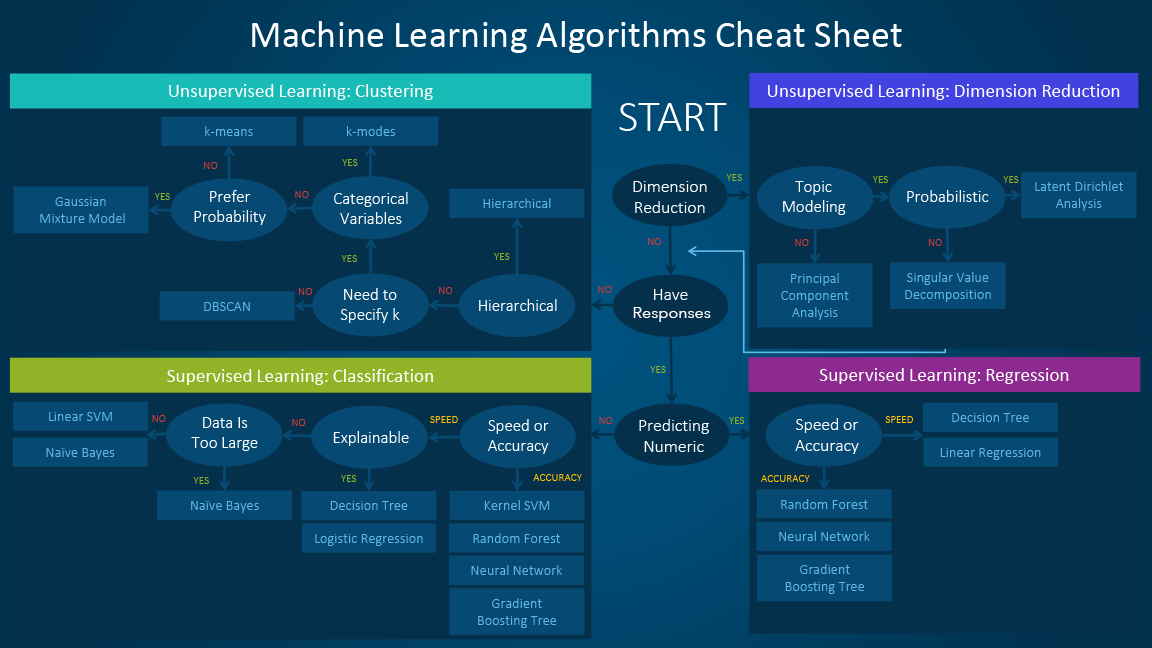
\includegraphics[width=150mm]{./appendices/machine-learning-cheet-sheet-2}
    \caption{Machine learning cheatsheet for algorithm choosing\cite{li2017mlalgorithm}
    \label{fig:ml-algorithm-cheatsheet}}
\end{figure}

This study focuses on anomaly detection,
which, simply put, is a clustering problem
where anomalies are rare incidents outside common clusters.
However,
in this study we utilize a PCA-based anomaly detection algorithm,
where PCA refers to Principal Component Analysis,
and which is a dimension reduction algorithm.~\cite{li2017mlalgorithm}
PCA is discussed in more detail later in this section.
In addition,
we aim to find a connection between anomalies and incident tickets
by their amount in a timeframe,
which makes the topic in the end a regression problem.

Typically,
the data used in algorithm training
is divided in two parts.
One part is used for the training process,
and the other is used to validate the results of the training.
These data parts must not overlap,
but the algorithm is given data to validate
that it has not seen before.~\cite{baheti2022datasplit}
For example,
in supervised learning
the key values the algorithm is trained to find
are hidden in the validation data.
The resulting values produced by the algorithm
are compared to the hidden values
and the difference between the estimate and the real value
can be used to determine how well the current trained algorithm compares to others.
However, in this study,
we are going to break that rule
of non-overlapping training and validation data.
The reason for this is explained further in section~\ref{subsec:pipe-unconventional-training}.

%% ************************************************************************************************************


\subsection{Cloud ML platforms}\label{subsec:bg-cloud-ml-platforms}

Machine learning algorithms are not light to operate.
ML is at its best with big data
where the large amount of data points
makes it easier for algorithms
to find repeating patterns more reliably.~\cite{zhou2017machine}
Data amount, however,
requires huge resources in terms of memory and computing power.
Especially with online applications
where real time analysis of new input data is required
with small latency,
cloud computing can make a big difference
in terms of processing speed.

The online market offers several solutions for ML computing in cloud.
Most notable service providers for
MLaaS (Machine Learning as a Service)
are Google, Amazon, IBM, and Microsoft.
Differences of each service provider are listed in table~\ref{fig:mlaas-comparison}.

\begin{figure}[htb]
    \centering
    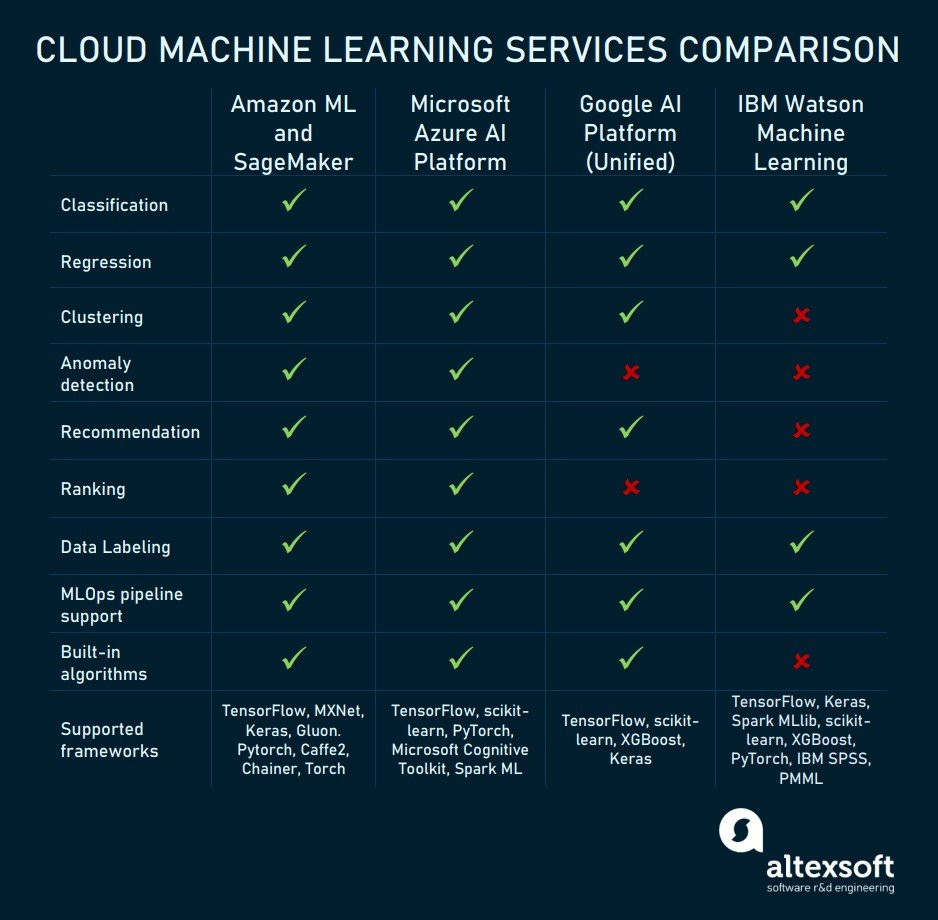
\includegraphics[width=150mm]{./appendices/mlaas-comparison}
    \caption{Machine learning as a Service comparison.~\cite{altexsoft2021mlaas}
    \label{fig:mlaas-comparison}}
\end{figure}

Amazon's new SageMaker service
has replaced the old Amazon Machine Learning service,
and is very much like Azure Machine Learning service
produced by Microsoft.
Compared to SageMaker and Azure, the
Google AI Platform is missing anomaly detection and ranking abilities.
IBM Watson has even less features,
as demonstrated in table~\ref{fig:mlaas-comparison}.~\cite{altexsoft2021mlaas}

Azure, however,
has one major advantage compared to SageMaker and other competitors,
which is the UI environment of ML Studio.
Most of the MLaaS providers' solutions
have some sort of no-code to low-code design features
which makes pipeline designing easy.
Azure ML Studio lets the developer design and deploy
full ML pipelines with drag-and-drop user interface.~\cite{altexsoft2021mlaas,microsoft2022azureml}

\begin{figure}[htb]
    \centering
    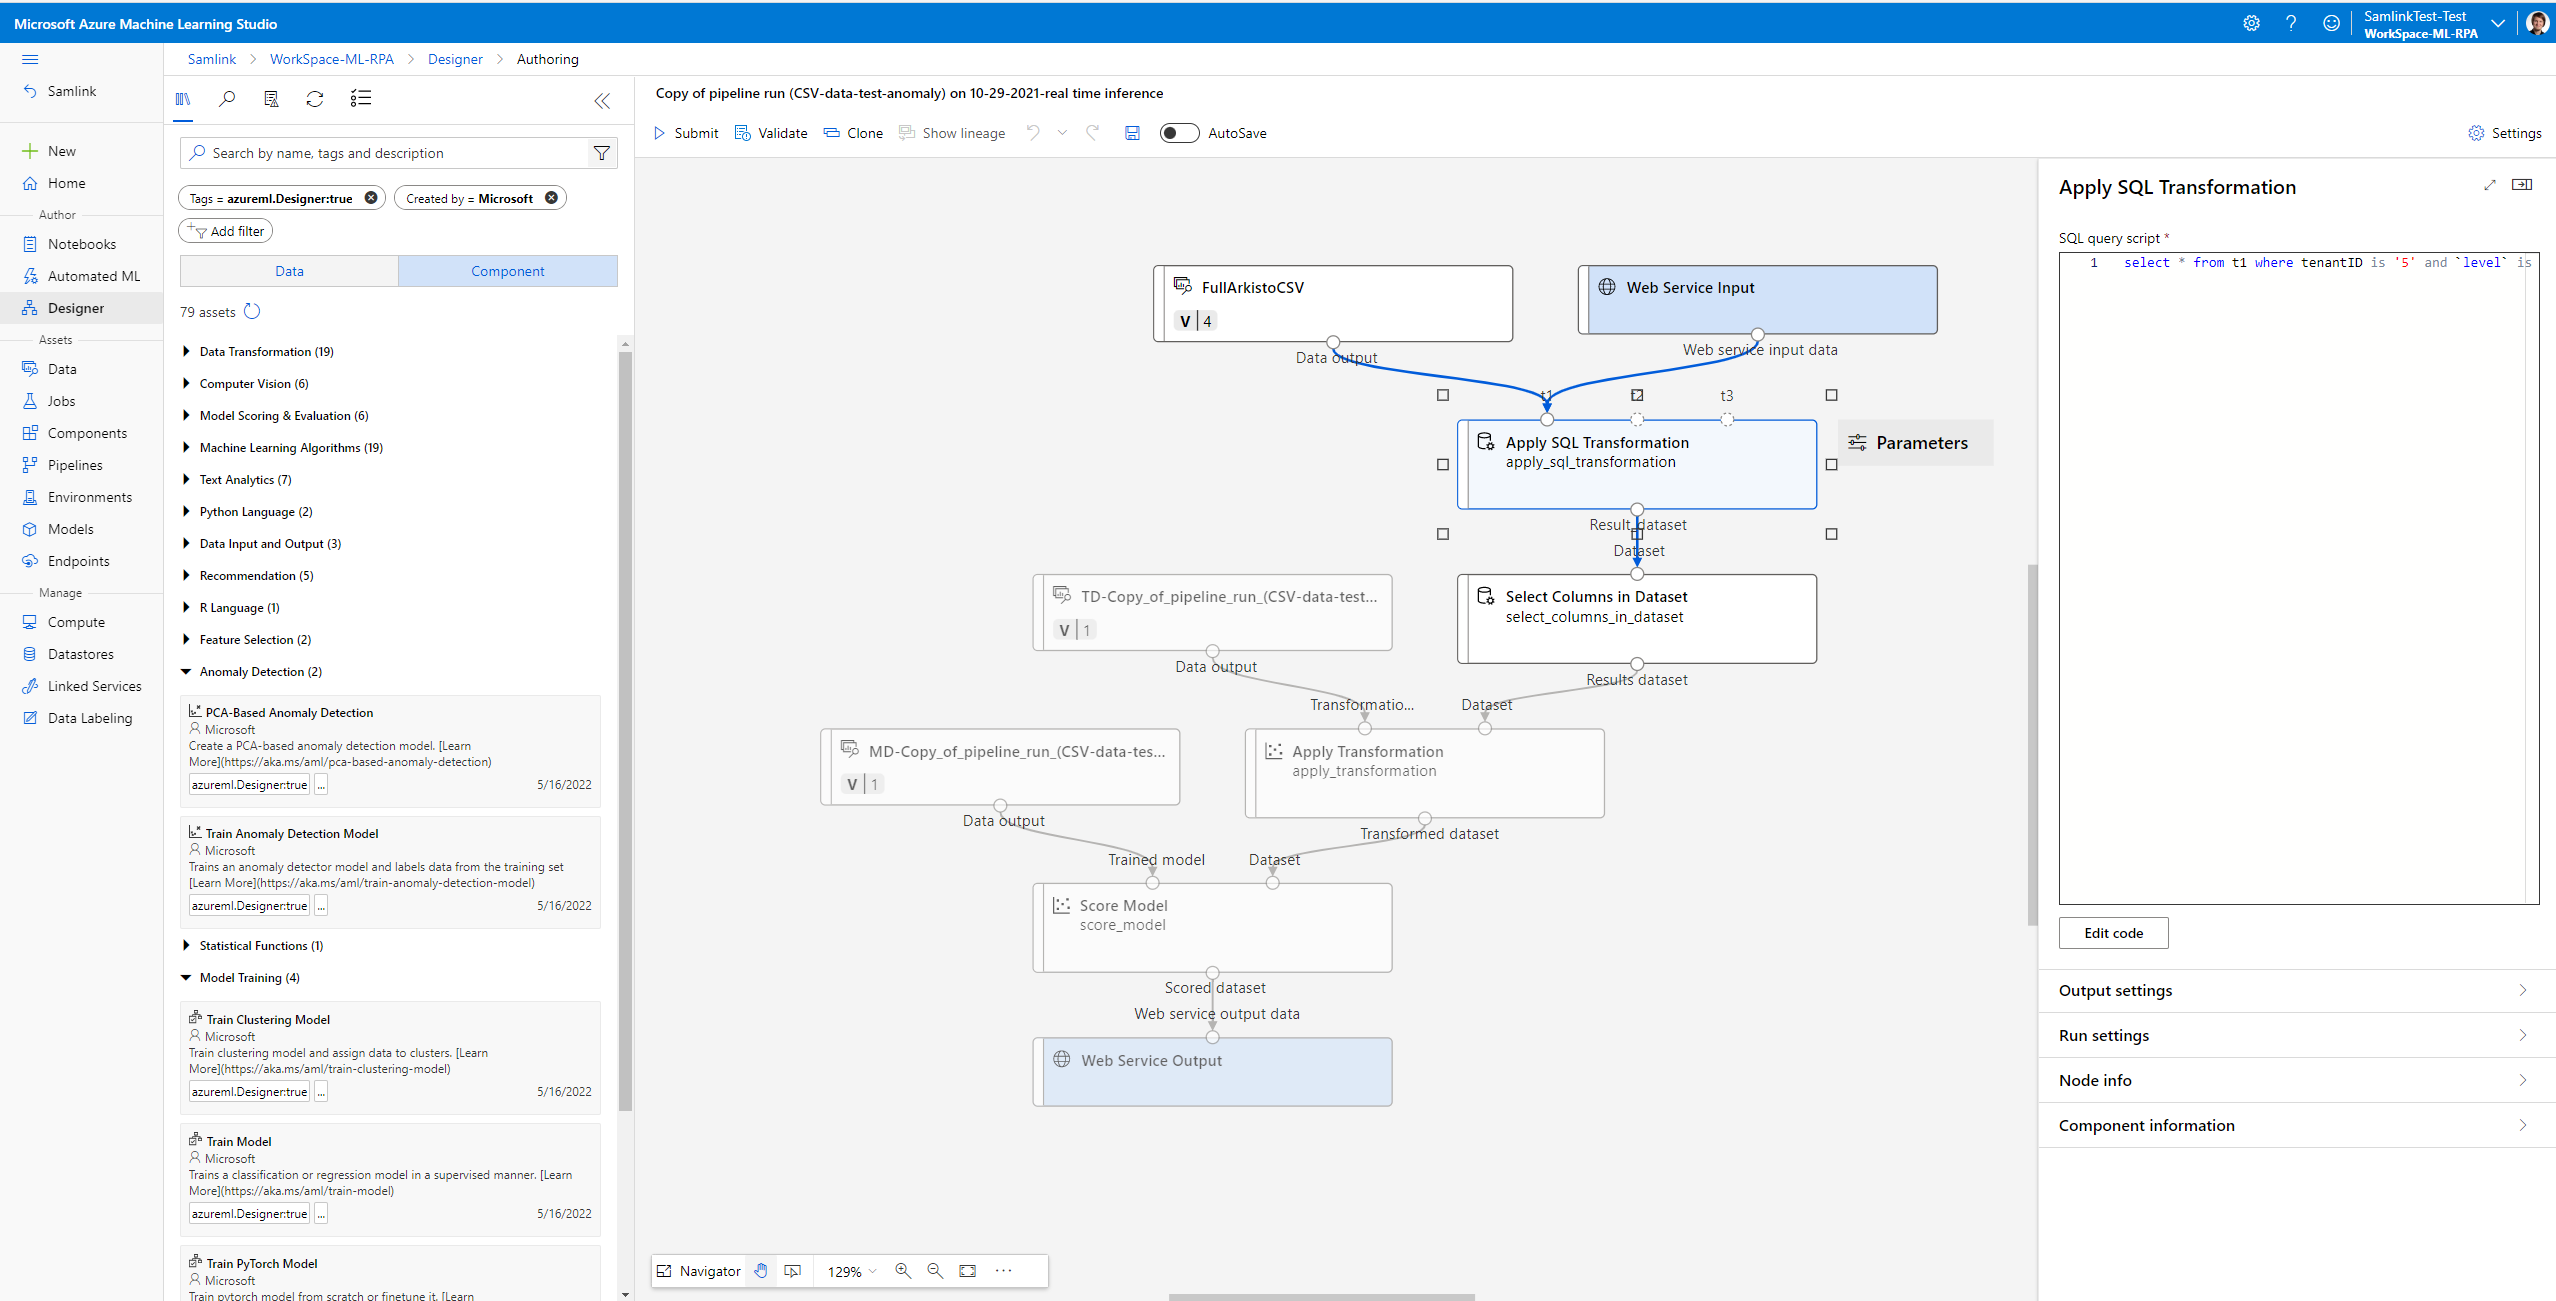
\includegraphics[width=150mm]{./appendices/azure-ml-studio-example}
    \caption{With drag-and-drop pipeline designer
    it is easy to get started with ML programming in Azure ML Studio,
    and visualizing the process helps understand all pipeline components
    and their relations to each other.
    \label{fig:azure-ml-studio-example}}
\end{figure}

Each component in the pipeline designer can be tuned
to certain extent.
ML Studio has a predefined set of ready algorithms to use.
An example of Azure ML Studio interface
is shown in figure~\ref{fig:azure-ml-studio-example}.
Data to the ML Studio environment
can be imported from local storage,
but also from various other Azure services
such as storage accounts with table and blob data.
Trained ML pipeline can be published as a cloud endpoint
and inserted into a wider operation chain
combining it with other Azure services,
like data storages and cloud computing resources.
This allows the designer to use ML computing capabilities
with existing production environments
utilizing services such as IoT, API, or Kubernetes.


%% ************************************************************************************************************

\subsection{Regression analysis}\label{subsec:bg-regression-ml}

Regression analysis is a typical approach in statistical science,
and thus, in machine learning too.
Algorithms based on regression analysis
are used to find relationships between a set of variables,
providing the means to \enquote{predict values of one variable
when given values of the others}
making them a fundamental component in the ML field.~\cite{merriam2022regression}

Regression algorithms intend to create a mathematical model
that explains the relations of the data.
This usually means an algebraic equation
which can be generalized in the following form,
\begin{equation}
    \label{eqn:general-regression-model}
    Y = f(X_{m},\beta_{p})+\epsilon
\end{equation}
where Y is the data feature we are looking to find relation to,
$f$ is some function of $m$ independent variables $(X_{m})$,
and $p$ coefficients $(\beta_{p})$.
$X_{m}$ can be opened as $X_{1},...,X_{m}$,
and $\beta_{p}$ as $\beta_{1},...,\beta_{p}$.
Note, that $m$ and $p$ do not have to be equal.
A single $X_{i}$ refers to a value of $i$th data row.
The $\epsilon$ refers to error term.
The goal is to determine the coefficients $\beta_{p}$
in order to find a model that explains the data.~\cite{freund2006regression}

As an example,
one of the best known principles for coefficient value solving
is the least square principle,
which aims to minimize the sum of squared errors (SSE).
The smaller the $SSE$ is,
the closer each data point is to the suggested model,
and the better the model explains the data
and can be used to make predictions.
The equation to solve in the least square principle
derived from the generalized form,
\begin{equation}
    \label{eqn:sum-of-squared-errors}
    SSE = \Sigma\epsilon^{2} = \Sigma[(Y-f(X_{1},...,X_{m},\beta_{1},...,\beta_{p}))]^{2}.
\end{equation}
Exact solution for this does not usually exist
as there can be more coefficients than independent variables $(p>m))$,
and minimizing the $SSE$ does not always result into a linear equation.
This is typically the case in ML,
and thus the model must be found
by iterative search process.
As mentioned in the section~\ref{subsec:bg-machine-learning},
this is what algorithms are build for.

To improve the efficiency of algorithm calculations,
the general regression model can be converted into matrix form.
The same function in equation~\ref{eqn:general-regression-model}
can thus be represented as,
\begin{equation}
    Y = XB+E
\end{equation}
where $Y$ is an $n\times1$ matrix of values in the data,
$X$ is an $n\times(m+1)$ matrix of independent variables,
$B$ is an $(m+1)\times1$ matrix of unknown coefficient parameters,
and finally, $E$ is an $n\times1$ matrix of error parameters.
Thus, the equation of squared errors (equation~\ref{eqn:sum-of-squared-errors})
that is to be minimized can be written as
\begin{equation}
    E^{T}E = (Y-XB)^{T}(Y-XB) = Y^{T}Y-2B^{T}X^{T}Y+B^{T}X^{T}XB.
\end{equation}
In order to minimize this, we can take the derivative of matrix $B$,
\begin{equation}
    \frac{\partial(E^{T}E)}{\partial B} = -2X^{T}Y + 2X^{T}XB
\end{equation}
and equating to zero gives
\begin{equation}
    (X^{T}X)\hat{B} = X^{T}Y.
\end{equation}
The solutions of coefficient parameters are thus
\begin{equation}
    \hat{B} = (X^{T}X)^{-1}X^{T}Y.
\end{equation}

Ultimately,
there usually is no one perfect model to describe real world data.
As an example,
the function $f$ in the general regression model
can describe the relation of $X_{i}$ and $\beta_{i}$ as a product of both terms.
This would mean, that
\begin{equation}
    f(X_{1},...,X_{m},\beta_{1},...,\beta_{m})=\beta_{0}+\beta_{1}x_{1}+...+\beta_{m}x_{m}
\end{equation}
which would be a linear regression model.
Example of an algorithm using this method
is visualized in figure ~\ref{fig:linear-regression-example}.
However,
real world problems cannot always be explained with a linear model.
Fitting a polynomial curve to the data
may improve the results of regression to a certain degree,
but it also has its limits.

\begin{figure}[htb]
    \centering
    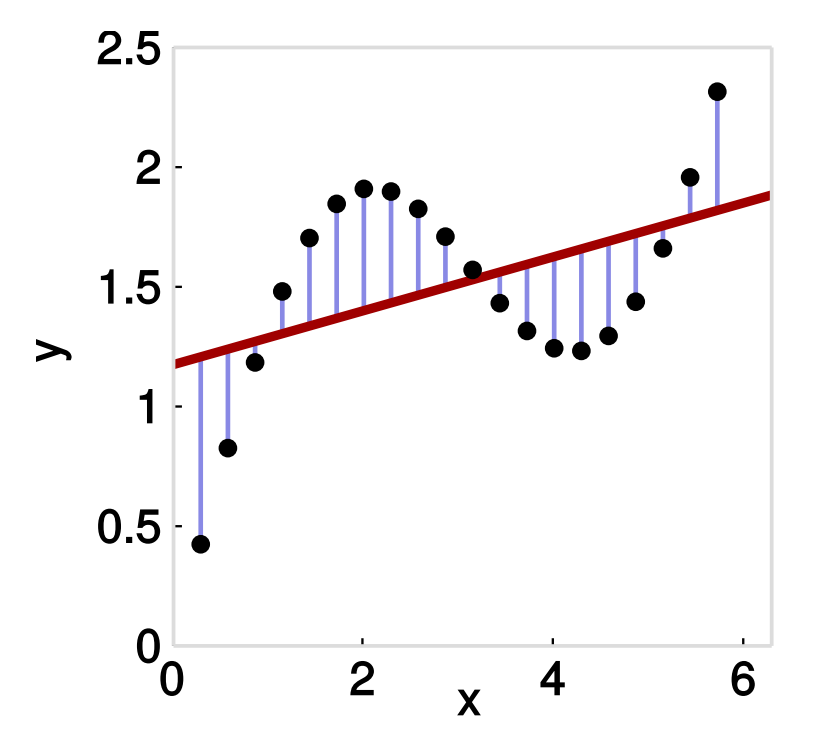
\includegraphics[width=0.5\textwidth]{./appendices/linear-regression}
    \caption{Linear least squares algorithm.
    Algorithm tries to fit a linear model (red line) on the data points,
        represented by the black dots,
        by minimizing the difference between all the data points
        and the model estimate.~\cite{stulp2015many}
        \label{fig:linear-regression-example}}
\end{figure}

Consider an algorithm that tries to keep a car
driving on a straight road in its lane.
The model output is how much we should turn the steering wheel
based on how much we are off from the straight line.
We might have constant parameters such as
wind effect, continuous error of the wheel axes, and tilt of the road.
However,
we also have parameters that change over time
and are dependent on other factors,
such as the weight of the car,
and the temperature and wear of the tires.
Therefore, with the same location at the road,
same car and same weather conditions,
our result could be different
depending on how long has been driven before the current moment
which affects the tire temperature and thus pressure.
Finding a model that best fits the data
depends also on the type of problem.
There are numerous algorithms to suit different situations,
and usually the best algorithm can be found
only by trial and error.


%% ************************************************************************************************************

\subsection{PCA-based anomaly detection}\label{subsec:bg-pca-ada}

Principal Component Analysis, or PCA,
is a machine learning technique
used to analyze data and explain the variance in it.
PCA analyzes data with multiple variables
and looks for correlations among them.
The final output PCA gives
is a new feature space,
\ie a smaller set of features (variables),
called \textit{principal components}.~\cite{azure2022pca}

In other words,
PCA works by reducing the dimensionality of the data.
First,
data must be standardized
so that the mean of each variable is zero
and the scale of each feature is the same.
\begin{equation}
    Standardized\; data\; point = \frac{data\; point\; value - mean\; value\; of\; the\; feature}{standard\; deviation\; of\; the\; feature}
\end{equation}
In practice,
the data points of each variable, or column,
is shifted so that their center is at 0
and the scale is adjusted to match all the variables.

Next, a covariance matrix for all the columns is determined.
As it is known,
covariance value between variables (or dimensions)
is calculated with
\begin{equation}
    cov(X,Y) = \frac{\Sigma_{i=1}^{n}(X_{i}-\bar{X})(Y_{i}-\bar{Y})}{(n-1)}
\end{equation}
where $X$ and $Y$ are different columns or variables,
$\bar{X}$ and $\bar{Y}$ their mean values (which both are zero after standardization),
$n$ is the number of rows or values in the data,
and so $X_{i}$ is the $i$th data point in the column $X$.~\cite{smith2002tutorial}

Covariance matrix is formed
by calculating the covariance value between each of the dimensions (including self).
For example,
for 3 dimensional data with dimensions $x$, $y$, and $z$, the
covariance matrix would be
\begin{equation}
    C =
    \begin{pmatrix}
        cov(x,x) & cov(x,y) & cov(x,z) \\
        cov(y,x) & cov(y,y) & cov(y,z) \\
        cov(z,x) & cov(z,y) & cov(z,z)
    \end{pmatrix}.
\end{equation}
Generally,
the covariance matrix for $n$ dimensions would then be, of course
\begin{equation}
    C =
    \begin{pmatrix}
        cov(1,1)    & \cdots    & cov(1,n)    \\
        \vdots      & \ddots    & \vdots        \\
        cov(n,1)    & \cdots    & cov(n,n)
    \end{pmatrix}.
\end{equation}

Next, we find the eigenvectors and eigenvalues
for the square-shaped covariance matrix.
As defined,
for $n\times n$ dimensional matrix $A$,
if exists a vector $x$ that satisfies
\begin{equation}
    Ax = \lambda x,
\end{equation}
where $\lambda$ is a scalar value,
such vector $x$ is an \textit{eigenvector} of matrix $A$,
and $\lambda$ is an \textit{eigenvalue},
forming the \textit{eigenpair} of $(\lambda,x)$.~\cite{borm2012numerical}

Eigenvectors have a property,
that either a matrix has zero of them,
or there are $n$ eigenvectors for $n\times n$ dimensional matrix.
Because in this case the eigenvectors are for the covariance matrix of the original (standardized) data,
they actually create a new feature space made of principal components.
More over, %% TODO: Continue grammar here Julia
eigenvalues describe their importance,
so that the greater the eigenvalue is,
the more significant the eigenvector is describing the original data
in principal component feature space.
When finding eigenpairs,
we actually find the largest possible variance in the data.
Each eigenvector describes a principal component
that is a linear combination of the original variables.
In the picture~\ref{fig:pca-example} we can see an example of
how eigenvectors of the covariance matrix define a new axis system
or new feature dimensions.~\cite{zhu2019dimension}
Each eigenvector, or a principal component,
is perpendicular with one another.
Thus, data can be represented
in the new axis system formed by eigenvectors.

\begin{figure}[htb]
    \centering
    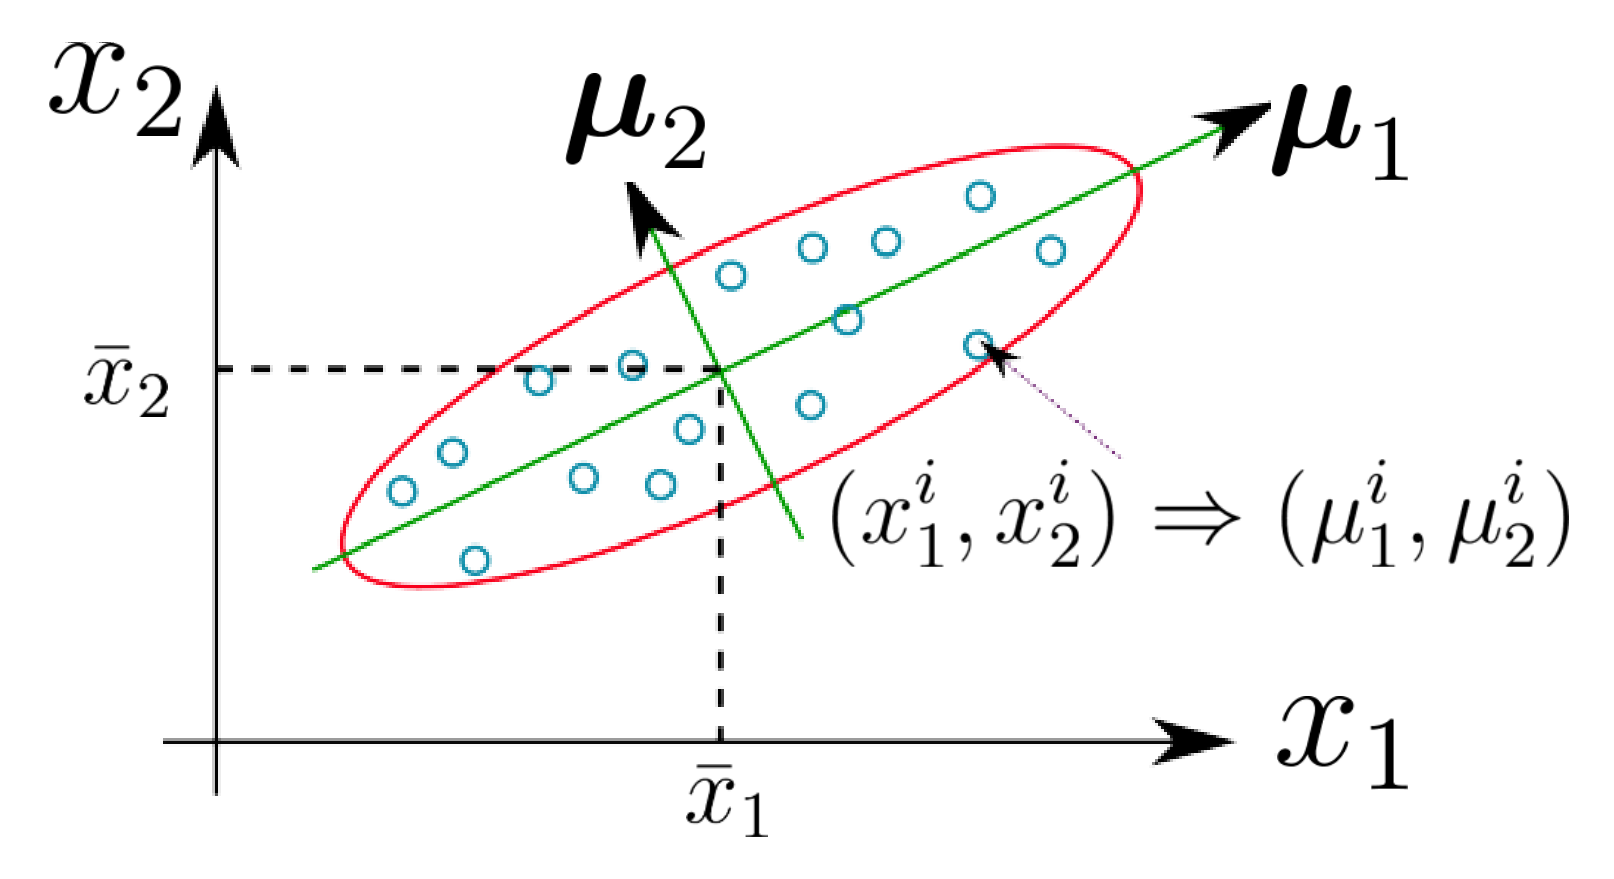
\includegraphics[width=0.7\textwidth]{./appendices/pca-example}
    \caption{Principal components form a new axis system.
    In this two dimensional example,
        eigenvectors $\mu_{1}$ and $\mu_{2}$ of the covariance matrix
        define new feature dimensions.
        Thus, data point $(x_{1}^{i},x_{2}^{i})$ of dimensions $x_{1}$ and $x_{2}$
        can be presented as a point $(\mu_{1}^{i},\mu_{2}^{i})$ of the dimensions $\mu_{1}$ and $\mu_{2}$.
        The origin point of each principal component axis is at the mean values of the data ($\bar{x}_{1}$ and $\bar{x}_{2}$)
        as the data is standardized.
        ~\cite{zhu2019dimension}
        \label{fig:pca-example}}
\end{figure}

By comparing the eigenvalues,
we can determine a set of eigenvectors,
or principal components,
that form a new feature space with fewer dimensions than original data,
without losing significant amount of information.
We can calculate a comparison value for each eigenvalue $\lambda_{i}$ with
\begin{equation}
    Percentage\; of\; variance = \frac{\lambda_{i}}{\Sigma\lambda}\cdot100
\end{equation}
Organized from highest to lowest,
we can make a scree plot to visualize their relationship.
Example of an 8 dimensional data,
thus 8 principal components,
with their eigenvalue variances ordered
can be seen in a picture~\ref{fig:pc-variance-values}.

\begin{figure}[htb]
    \centering
    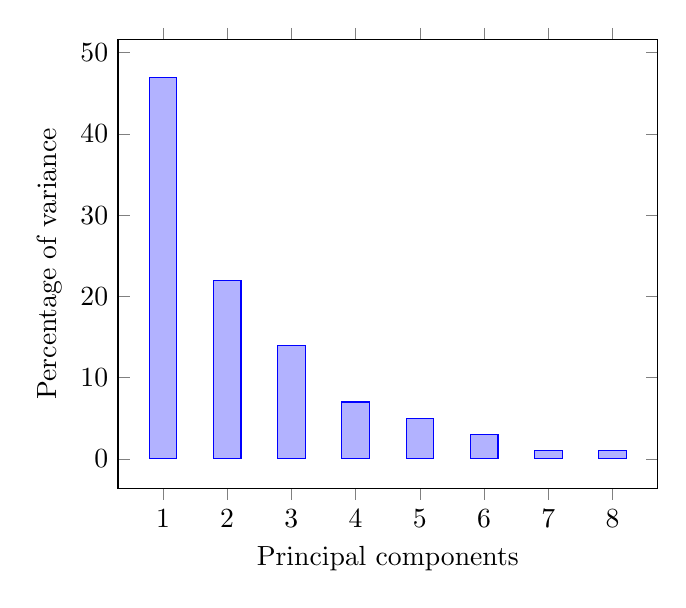
\begin{tikzpicture}
        \begin{axis} [
            ybar,
            ylabel={Percentage of variance},
            xlabel={Principal components},
            symbolic x coords={1,2,3,4,5,6,7,8},
            xtick=data
        ]
            \addplot coordinates {
                (1,47)
                (2,22)
                (3,14)
                (4,7)
                (5,5)
                (6,3)
                (7,1)
                (8,1)
            };
        \end{axis}
    \end{tikzpicture}
\caption{Principal components significance.
In this example, eigenvalues, or the variance of each principal component,
    are ordered on a scree plot.
    Values are first converted to a percentage of the sum of all values
    in order to visualize both their relationship to each other
    and their total share of information the corresponding eigenvectors hold.
    \label{fig:pc-variance-values}}
\end{figure}

Practically,
as principal component space describes the data
and eigenvalues describe the importance of each component,
the percentage of variance is the portion of the total information each principal component holds.
Simply put,
in our example picture~\ref{fig:pc-variance-values},
first two principal components hold almost 70\% of the original information,
first three over 80\%,
and last seven hold less than 20\% of the information.
Thus,
by creating a new data set using first three components,
we can keep 80\% of the information
while reducing the dimensions from 8 to 3,
which would be significant improvement
in terms of computing resources needed.
The amount of top principal components we choose to keep
depends on the situation,
but one guideline is to select all components
that describe more than a single variable's worth of information.
For our 8 dimensional example,
that would mean $1/8$th, or $12.5\%$,
meaning that we would select top 3 principal components
and discard the rest that are under $12.5\%$ of variance.
The remaining vectors form a new matrix
called \textit{feature vector}:
\begin{equation}
    Feature\; vector\; (F) = (x_{1} x_{2} ... x_{p})
\end{equation}
where $x_{i}$ is the $i$th eigenvector or feature component we chose to keep,
and $p$ is the amount of them, where $p<n$, $n$ being the original amount of dimensions of the data.

Finally,
we reorient our data from the original axes
to the space defined by the principal components
with the following equation:
\begin{equation}
    Final\; data = F^{T} A^{T}
\end{equation}
where $A$ is the original data set with standardized data,
which is transposed as well as the feature vector multiplying it.\cite{jaadi2021pca,holland2008principal,smith2002tutorial}

With principal components describing the distribution and variance of the data majority,
we can use PCA to detect anomalies.
This is done by analyzing each input
and computing its
\enquote{projection on the eigenvectors,
    together with a normalized reconstruction error.
    The normalized error is used as the anomaly score.
    The higher the error, the more anomalous the instance is}~\cite{azure2022pca}.
Normalized error means,
that each anomaly score is between zero and one.


%% TODO: picture of anomaly detection with PCA?

%% ............................................................................................................

\subsection{Other anomaly detection algorithms}\label{bg-other-ada}

Azure ML Studio has,
or used to have,
also another anomaly detection algorithm to use besides PCA-based one.
This module is called One-Class Support Vector Machine.
However,
it was not usable in the renewed ML Studio environment,
but was only available in the \textit{classic} Azure ML Studio.
In addition,
this module was not deemed suitable in our case,
as the documentation mentioned that
\enquote{The dataset that you use for training
can contain all or mostly normal cases.}
Because the content of the data used did not meet this requirement,
the usage possibilities of this component were not decided to investigate.~\cite{azure2021oneclasssvm}
To limit the scope of this study to reasonable proportions,
we will not discuss other anomaly detection algorithms (ADAs) further.

%% ************************************************************************************************************

\subsection{N-gram features and feature hashing}\label{subsec:bg-ngram-features-and-hashing}

As discussed before,
features are the key elements in ML algorithm training.
As textual input does not have any meaning to computers as itself,
it is necessary to create a connection between words and features for algorithm.
In ML training,
one typical approach is to convert textual input to numerical features.
For example, by creating a dictionary of words used in the input
and assigning each word an identification number,
we can express sentences as a count of certain words used.
In addition,
words include meanings not only individually but also
with relation to each other and with their order.
For example,
words "success without errors"
has the opposite meaning than "errors without success"
where same words exist in a different order.
We can add more information for the algorithm
by creating word pairs and groups in the dictionary.
These groups are referred as word grams,
where \textbf{n} in n-gram refers to the maximum number of words
in a group of consecutive words in the input sentence.~\cite{furnkranz1998study}

Example of n-gram composition of a sentence can be seen
in the table~\ref{tab:bg-n-gram-example}.
Usually,
the unnecessary stop words are removed from the text
(such as "the"),
as they don't bring any additional meaning to words or sentence.
One word grams are called \textit{unigrams},
two word grams \textit{bigrams}, \etc.
To compose the sentence \textit{"Lorem ipsum dolor sit amet, quisquam est, qui dolor ipsum qui dolor sit amet"}
with different n-gram dictionaries,
we could make, for example,
the following presentation with unigram dictionary:
\begin{equation}
    1,2,3,4,5,6,7,8,3,2,8,3,4,5
\end{equation}
where each number represents the index of a word in unigram dictionary from table~\ref{tab:bg-n-gram-example}.

\begin{table}[htb]
    \begin{tabularx}{\textwidth}{|L{0.1\textwidth}|L{0.17\textwidth}|L{0.25\textwidth}|Y|}
        \hline
        \textbf{Index} &
        \textbf{Unigrams} &
        \textbf{Bigrams} &
        \textbf{Trigrams}
        \\ \hline
        1	&	lorem       &	lorem ipsum     &	lorem ipsum dolor  \\ \hline
        2	&	ipsum       &	ipsum dolor     &	ipsum dolor sit  \\ \hline
        3	&	dolor       &	dolor sit       &	dolor sit amet  \\ \hline
        4	&	sit         &	sit amet        &	sit amet quisquam  \\ \hline
        5	&	amet        &	amet quisquam   &	amet quisquam est  \\ \hline
        6	&	quisquam    &   quisquam est    &	quisquam est qui \\ \hline
        7	&	est         &   est qui 		&	est qui dolor  \\ \hline
        8	&	qui         &   qui dolor 	    &	qui dolor ipsum \\ \hline
        9	&	            &  	dolor ipsum 	&   dolor ipsum qui \\ \hline
        10	&	            &  	ipsum qui 		&   ipsum qui dolor \\ \hline
        11	&	            &  	 				&   qui dolor sit \\ \hline
    \end{tabularx}
    \caption{N-gram feature extraction from a sentence
    "Lorem ipsum dolor sit amet, quisquam est, qui dolor ipsum qui dolor sit amet".}
    \label{tab:bg-n-gram-example}
\end{table}

N-gram representation of the text
streamlines the algorithm processing of textual features.
However,
each new word creates a new feature
when converting text to n-grams.
This happens,
because in order to present text as numerical features,
we need to create a new feature space out of the n-gram dictionary.
Consider our unigram dictionary from the previous example.
This would convert one text column into 8 unigram features,
as seen in the table~\ref{tab:bg-n-gram-features}.

\begin{table}[htb]\small
\begin{tabularx}{\textwidth}{|L{0.07\textwidth}|L{0.09\textwidth}|L{0.09\textwidth}|L{0.08\textwidth}|L{0.07\textwidth}|L{0.07\textwidth}|Y|L{0.07\textwidth}|L{0.07\textwidth}|}
    \hline
    \textbf{row} &
    \textbf{lorem} &
    \textbf{ipsum} &
    \textbf{dolor} &
    \textbf{sit}	&
    \textbf{amet} &
    \textbf{quisquam} &
    \textbf{est} &
    \textbf{qui}
    \\ \hline
    1	&	1	&	2	&	3	&	1	&	2	&	1	&	1	&	2 \\ \hline
\end{tabularx}
\caption{One row with a textual feature presented as n-gram feature transformation.
Each new word in the n-gram dictionary adds a new feature and thus a dimension to the data.}
\label{tab:bg-n-gram-features}
\end{table}

As the number of word grams in a dictionary can increase significantly
in complex input cases,
it is necessary to limit the resource usage by decreasing the features analyzed.
In order to compress the dimensions,
one way is to use feature hashing for n-gram features.~\cite{azure2021fhash}
This means that instead of pure n-gram features representing a single n-gram instance,
we use hashed value of several n-grams
thus reducing the amount of features.
Hashing can be done in different ways,
for example by multiplying each original feature together,
or calculating a weight value based on the frequency of each feature.
As a drawback,
the amount of information might also get reduced as the data is "compressed".
The more dimensions are compressed into hashing values,
the more information is bound to be lost,
but this way we can include more features for algorithm training
without significant resource demands.~\cite{caragea2012protein,shi2009hash}

%% ************************************************************************************************************

\subsection{Robotic process automation}\label{subsec:bg-rpa}

Robotic process automation, or RPA,
is used to automate mechanical tasks executed on computer software.
Usually it operates on the UI level
and can be used to repeat meaningful functions
instead of mechanical actions.
For example, with screen recording macros
only position at the screen and mechanical key pressing is recorded and repeated.
RPA automation, however,
is able to repeat the functionalities those actions trigger,
such as inputting text to a certain named field on the UI,
or logging in with given username and password
regardless of the location of those fields on the layout.~\cite{tripathi2018learning}

In Samlink,
an RPA technology called UiPath is used as a base of RPA operations.
A central coordinating system called \textit{UiPath Orchestrator}
supervises the RPA processes.
RPA process is executed by following
an \textit{RPA automation},
a predefined operation instruction build by RPA developer.
The software responsible of the automation execution
is called an \textit{RPA agent}.
Agents are located in the \textit{workstations},
where a single agent is running in one workstation.
Each agent executes one automation at a time,
given by the Orchestrator,
and communicates with Orchestrator during the execution.
This hierarchy is visualized in the picture~\ref{fig:rpa-hierarchy}.

\begin{figure}[htb]
    \centering
    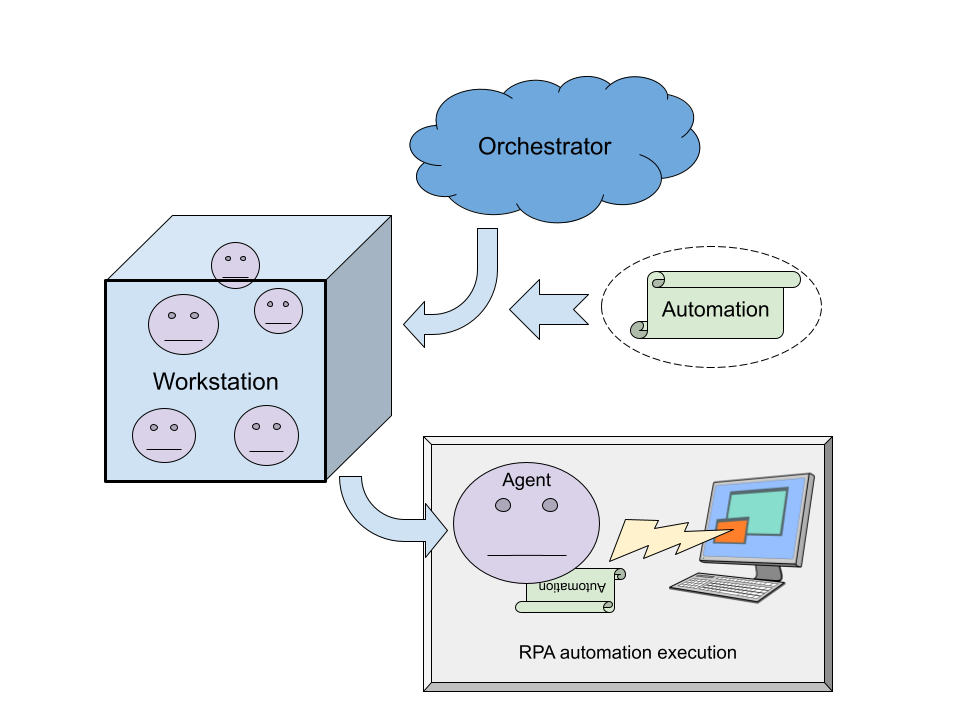
\includegraphics[width=\textwidth,]{./appendices/RPA-hierarchy}
    \caption{Hierarchy of RPA components explaining the terms and their relations.
    \label{fig:rpa-hierarchy}}
\end{figure}


%% ************************************************************************************************************

\subsection{Data sensitivity}\label{subsec:bg-data-sensitivity}

During this study,
it was necessary to make sure no sensitive data
was moved out of the production environment.
This was mostly due to restrictions imposed by GDPR\@.
In order to maintain the data security,
data had to be anonymized
before it could be exported to the cloud environment.
After anonymization,
data would not include any information
that can be connected to real individuals.
Three different anonymization methods were considered,
which were pseudonymization, k-anonymization and full anonymization.

Pseudonymization refers to a method
where sensitive information is de-identified.
This means,
that each sensitive piece of information
is replaced with an encrypted value
so that no information is lost
but human cannot identify individuals
when reading the data.
Encryption and de-identification
could be reversed, \ie data could be re-identified,
with decryption key which tells computer
how to convert the replaced value back to the original form.
As machine learning algorithms do not care about the meanings
behind personal identification information,
such as phone numbers or addresses,
pseudonymization would preserve the information in the data unchanged
for ML algorithms to use so that no information would be lost.~\cite{noumeir2007pseudonymization}

As pseudonymization is reversible operation with encryption key,
it is not the safest way to anonymize the data
because encryption key leaking is always a risk.
K-anonymization is the next step to secure the data sensitivity.
Excluding all unique identifiers such as full name or social security number,
information like home street, age, workplace or last name
are not on their own enough to identify certain individual,
but combined they can single out a person.
K-anonymization is unreversable anonymization approach
where identifying information is generalized
to mask individuals into crowd.
With k-anonymization,
algorithm replaces single informative details
with more general variants,
for instance,
address to hometown or age to age range.
K-anonymization loses information
as it cannot be reversed.
If personal information is essential for the use case of ML algorithm,
this method weakens the algorithm results.~\cite{byun2007efficient}

Eventually,
due to high customer data sensitivity and strict data safety policies,
it was determined that individual information in the log data used in this study
was not relevant for connecting the log events to technical support ticket timestamps,
and full anonymization was decided to execute on the log data.
This way,
each personal information was replaced with a general token
disclosing only what type of information (phone number, email address \etc) was anonymized.
Frankly,
it was not certain if identifiable personal data had improved algorithm results,
but because corresponding support ticket data
was stripped from all other information except timestamps,
any possible connections between personal data in logs and in tickets
were lost in any case.

Data anonymization was executed in production environment
with PowerShell script.
Several predefined identification features were searched with
regular expression (or regex) patterns and replaced with
default keys.
Anonymization scripts and data format
is described more in the section~\ref{subsec:meth-data-anonymization}.


%% ************************************************************************************************************

\subsection{Log data analyzing and anomaly detection with ML}\label{subsec:bg-log-data-analyzing-and-anomaly-detection-with-ml}

Using machine learning for log data analyzing
is not a new field of study.~\cite{rantala2019applying,allagi2019analysis,kondo2017early,cao2017machine}
Key issue tends to be the format of the log data
which shifts the dilemma to natural language processing.
Some studies also combine anomaly detection using machine learning
to log data analysis.~\cite{liu2019loganomaly, zhang2019robust}
Comparing existing studies to our case
raises at least one major suggestion for improvement:
log data refining.

When log data has consistent format,
multiple different algorithms can be utilized
for anomaly detection and log analyzing.
Log events can be clustered
and different types of events can be counted
if the amount of types is finite and known.~\cite{liu2019loganomaly}

If training data already have information
we wish to teach the algorithm to forecast (\ie data is labeled),
combining the results of the log data analysis to external features
is more feasible.
With labeled data,
supervised learning methods can improve the results of the algorithm forecast abilities.
~\cite{rantala2019applying}

As explained in the section~\ref{subsec:meth-efecte-ticket-data},
data features connected to anomaly detection results
are pure datetime values.
With more insight to ticket data properties than just timestamps,
ML algorithms could be able to extract more valuable information
from the log data.


\clearpage
%!TEX root = thesis.tex
%% %% ***************** Research materials and methods *****************

%% ************************************************ 3 ************************************************

\section{Research material and methods}\label{sec:research-material-and-methods}
%\section{Tutkimusaineisto ja -menetelmät}

In the next section
we explain in more detail
what the data used in the study
consists of
and what methods were used
in attempt to answer the research goals.

The data in the research is mainly made up of two parts.
The most important part is, obviously,
the log data produced by the numerous RPA processes.
The second part complementing the study
is the support ticket data written by clerks of customer banks.
In order to use the data safely in the cloud environment
it was necessary to sanitize the data
from any sensitive information.
This was done by anonymizing the log data
and using only timestamps from the support tickets.

%% ************************************************************************************************************

\subsection{Support ticket data}\label{subsec:meth-efecte-ticket-data}

Like all other software,
RPA components fail from time to time.
As described before,
RPA logs are verbose
making possible error identification from among it hard.
Due to that,
it is not feasible to create log parsers
that would be able to identify critical errors
from within thousands of lines of log.
When critical error happens
causing the RPA process to fail,
the banking clerks need to fix manually
the job left by the RPA process.
Every time this happens,
these clerks then send a support request ticket
to Samlink technical help desk
and ask to fix the issue.

When clerks send the ticket to technical support
a verbose description of the situation is written
to help developers to identify the problem.
This description often contains sensitive end customer information
like bank account details and social security numbers.
To avoid privacy issues when processing this data,
it was decided to use only timestamps of the tickets.
The resulting data was practically a list of date and time values.
More about the issue from privacy point of view
is described in section~\ref{subsec:meth-data-anonymization}.

%% ************************************************************************************************************

\subsection{RPA log data}\label{subsec:meth-rpa-log-data}
Robotic process algorithms used in Samlink
are designed
to ease the workload of bank clerks.
RPA robots
work mostly with loan applications
among other routine tasks
that require mostly manual labor.
\todo{Check!}

Like other software,
RPA also produces log data during runtime.
As several RPA robots are running
the amount of log produced daily is also significant.
\todo{How many RPA:s? How many customers? How much log data?}
%% TODO: How many RPAs
%% TODO: how many customers are they dealing with?
%% TODO: AMOUNTS!
This log data is not in consistent structure
being formed out of typical CSV data
injected with even more inconsistent JSON data
that varies in contents vastly.
\todo{refer to appendices, include examples of data}

RPA log data is stored in SQL database.
The database is split in live production log
that is gathered for few months
and then moved to archive that has
several years worth of log.
\todo{check live timescale}
%% TODO: Check

In this study we used archived data
as it was easier to acquire in one run
without the need to merge different parts together.
Archive also had
data that was considered as sufficient amount
for machine learning algorithm training.
\todo{how much really?}

\subsubsection*{Data formatting}\label{subsubsec:data-formatting}
At the beginning of the research,
the log data from RPA was in SQL database.
However,
the database used was not "pure"
in a way that typical relational databases are,
but some columns included JSON-formatted data in them.
For ML algorithms to be able to read the given data with ease
this kind of impurities needed to be cleared from the data.

When feeding the log data to anomaly detection algorithm
it was necessary that all the rows were
as minimally unique as possible
in order to use the pattern finding abilities of the algorithm.
Too unique data points would have made all of them anomalies
compared to each other.
Thus, all unique features were stripped from the data,
such as the fingerprint value
that was unique for each data point.
Also,
job ID information and timestamps of the rows
were removed momentarily.
\todo{check above section so it makes sense}
%% TODO: this was done with case:RawMessage
%% TODO: fix above to make sense

%% ************************************************************************************************************

\subsection{Data anonymization}\label{subsec:meth-data-anonymization}

\subsubsection*{Support ticket data privacy}
Samlink handles highly sensitive banking customer data in its processes,
such as personal identification numbers, home addresses, email addresses and bank account numbers.
All possibly sensitive data must be removed
before data can be transferred out from production environment to cloud.
Due to bureaucratic reasons,
technical support tickets were under more strict policies.
Because of this,
they were allowed to be used in the research
on condition that no business critical nor customer sensitive information
was processed in the first place.
Only way to assure this
was to select solely timestamp fields from ticket data.
Thus, no sanitation for ticket data was needed
as ticket data consisted of only list of datetime values.

\subsubsection*{RPA log data sanitization}
Information privacy is one of the key values in Samlink business promise
as company develops high security banking applications
and processes sensitive customer data.
Thus, several aspects were needed to take into consideration
before log data could be authorized for thesis study usage.
To improve privacy,
it was decided to assume
that personal customer details are not critical information
for ML algorithm training
if goal is to find possible problems in RPA runtime
and not detect individual customer related problems.
This way it was not necessary to achieve adequate security
by less secure and more effort consuming ways
such as pseudonymization or k-anonymization,
which would have also required strict inspections
before data could have been approved for cloud processing.
\todo{References?}
%% TODO: references?

As production environment is built on Microsoft Server based solution,
and because it was highly unrecommended
to install additional software to the production server,
data acquiring and anonymization tools were chosen
based on what was already usable in the RPA production environment.
Microsoft Powershell offers sufficient tools
for database SQL querying
and stream editing.
The amount of data was significant
which made straight file editing impossible
due to the memory limitations.
Thus, stream editing was necessary
for finding and replacing
sensitive information from the data.
\todo{maybe references?}
%% TODO: References!

Anonymization took good proportion of the time in workdays
as processes were slow,
amount of data was big
and multiple re-runs were needed
before the results was seemed adequate.
\todo{Appendix of the script used. Does this need more explaining?}
%% TODO: appendix of the script used

%% ************************************************************************************************************

\subsection{Azure environment}\label{subsec:meth-azure-environment}

\todo{This section is under construction! Here are some things we are discussing here:}
Azure resources, such as virtual networks, storage spaces, connections to ML studio \etc

More info about ML studio, WYSIWYG-programming (or drag'n'dropping components),
computing clusters, jobs, datasets and such.
What kind of resources were usable based on the issue at hand
and limitations by the company (cost, basically).

%% TODO: <Azure resources, virtual network etc.>
% Several different ML methods are usable with Azure ML Studio.
% %%TODO: open up


%% ************************************************************************************************************


\subsection{Machine learning pipeline}\label{subsec:meth-ml-pipeline}

\todo{this section is under construction}
As stated in section~\ref{subsec:bg-ml-field},
the approach in this thesis is,
if expression is allowed, unorthodox.
Typically,
it is not a good idea to use
same data points in ML algorithm training and validating.
Acting otherwise
leads to algorithm processing with
same data it was trained with
thus creating a situation
where algorithm already knows what to do with the current datapoint.
If the results were validated after this
the algorithm would get unreliable score
as it had the validation data already in the training phase.
This could be compared to
giving some right answers to students
during test and scoring test results as if
no help wasn't given.

%% TODO: explain why we did it anyway!


Initial plan when starting the ML pipeline testing
was to feed the log data to anomaly detection algorithm
and try to get some sort of estimate of possible anomaly count.
This plan had several problems.

First, as stated, logging is very abundant
and several thousands of rows is logged
during a single day.
Some errors encountered are not critical
and RPA robot is able to recover from them
finalizing the initial task.
This means, that errors that could be deemed anomalous
may not result to a ticket in the end.

In addition,
one single error case
may be linked to several problems in runtime,
meaning that one ticket received is,
in fact, linked to multiple or
even dozens of log rows.


%% TODO: << logeissa päivän aikana yhteen tikettiin liittyen satoja rivejä
%% anomalioiden määrä voi olla tuhansia vaikka tikettejä vain kymmenkunta
%% ei kerro vertailukelpoista määrää

Two different algorithms are needed.
In phase 1,
algorithm defines how likely one datapoint
is to be considered an anomaly.
In phase 2,
another algorithm aims to predict
how many tickets are to be expected to receive
within a time frame.
Phase 1 is purely anomaly detection
while phase 2 could use
classification within time frame

Possible algorithms to consider in phase 2:
\begin{verbatim}
  Artificial Neural Network, reinforced learning
\end{verbatim}


%% TODO: unorganized text below!
Usually <with usual ml methods> the estimates
created using ML algorithms
are formed based on the certain features
presented on a one element of the data,
or on one row.
This means that in typical case,
there is one column in the data
given to the ML algorithm
that is removed from the training data
and this column value is what algorithm
aims to predict.

In this study case, however,
data does not contain clear values
that are being estimated
and that can be used as comparison.

\begin{tabular}{cccc}
    LOG\_DATA \\
    a=date & b=msg & c=\etc & \\
    a & b & c & n1 \\
    a & b & c & n2 \\
    a & b & c & n3 \\
    a & b & c & n4
\end{tabular}
\begin{tabular}{c}
    EFECTE\_DATA \\
    A YYYY.MM.DD hh:mm:ss \\
    B YYYY.MM.DD hh:mm:ss \\
    C YYYY.MM.DD hh:mm:ss \\
    D YYYY.MM.DD hh:mm:ss \\
    E YYYY.MM.DD hh:mm:ss
\end{tabular}
\\
n1 = SUM(AB) \\
n2 = SUM(C) \\
n3 = SUM(DE) \\
=> \\
We could try to predict nx
but usually this is done
by making estimate based on
a, b and c.
Instead,
we aim to estimate the sum of events
in timeframe.
We should also skip event instances
that are close to each other
to avoid counting multiple values
linked to same error
as different possible ticket creators.


\subsubsection*{Memory issues and limitations}
Memory is crucial in ML training
as multiple steps happen
and data is formatted \etc. %% TODO: fix!
While building ML pipeline in Azure ML studio,
a memory issue emerged
that affected several components
and caused serious limitations
in terms of usable components and data size.
Due to the time limits of this study
this issue was not resolved
and the problem behind it was not found.
As several conditions
considering the environment costs
were already issued by the company,
the issue was declared to be linked with
compute instance property limitations.
However, this was not certain.

%% TODO: limitations to components
%% limitations to data size
%% effects on choises in components?


\subsubsection*{Feature format for PCA-ADA}
%% TODO: n-gram vs pure data input
In Azure ML Studio
there is only one module selectable
for anomaly detecting,
the PCA-based anomaly detection module,
which is explained in section~\ref{subsec:bg-pca-ada}.
However,
with textual input like logs
it can be used at least in two ways.
First,
input data can be fed to
the algorithm trainer as is,
letting the PCA-based ADA component
do the work without further modifying the log rows.
This way,
the component tries to recognize the anomalies
based on all the information included in the row.
Practically this means
that the component processes data in textual format
making each row in the input
a feature as a whole
to consider.

Second option is to
convert the textual features
into numerical N-Gram features.
Each word or N-Gram %% TODO: Open up!
is now a number of said instances found on
the row being processed,
and each row can be presented
as a sequence of numbers
indicating the number of those features.

N-Grams can in addition have a weight
based on the frequency they appear
in the entire data.
Different weights usable in Azure ML component
are listed below

\begin{enumerate}
    \item Binary Weight
    \item TF Weight
    \item IDF Weight
    \item TF-IDF Weight
\end{enumerate}


\subsubsection*{Anomaly probability}
%% TODO: PCA output

\subsubsection*{Statistical features}
%% TODO: combination with ticket data. SQL queries


\subsubsection*{Regression based estimating}
%% TODO: parameters?
%% Ticket amount forecasting

\begin{enumerate}
    \item Linear regression
    \item Decision forest regression
    \item \etc
    \item \etc
\end{enumerate}


\clearpage
%!TEX root = thesis.tex
%% %% ***************** Machine learning pipeline structure *****************

%% ************************************************ 4 ************************************************

\section{Machine learning pipeline structure}\label{sec:ml-pipeline}

The full component chain from input to output
with algorithm training and result validating
is called a machine learning pipeline.
In this section,
we discuss how the ML pipeline was created in Azure ML Studio.
Several ML algorithms were compared
in order to find the most feasible set for our goal in mind.
ML training was organized in two different phases
in order to find the relation between
log anomalies and technical tickets.
Although, the Azure environment and ML Studio requirements
were the objectives of the study and therefore part of the outcome of the results,
these results were also a prerequisite for solving the final objective
considering the possibilities of the ML algorithm.
Therefore,
the resulting Azure resources and ML Studio pipeline components
are demonstrated in this section.

Results of the trained algorithms
were validated against newly acquired production data
in order to estimate how well the initial goals of the study
were fulfilled.
These results are presented later in the section~\ref{sec:results}.

Azure ML Studio makes ML pipeline creation easy
and comparing different methods and algorithms effortless.
Nevertheless,
with a hybrid approach having two different phases,
and result comparison being done against the anomaly hypothesis,
the pipeline drafts started to accumulate in content.

When starting the ML pipeline testing,
the initial plan was to feed the log data to the anomaly detection algorithm
and try to get some sort of estimate of possible anomaly count.
This plan had several problems.
First, as stated, logging is very abundant
and several thousands of rows is logged
during a single day.
Some encountered errors are not critical
and RPA agent is able to recover from them
and finalize the initial task.
This means,
that errors which could be deemed anomalous
may not result to a ticket in the end.

In addition,
one single error case noticed by bank clerks
may be linked to several problems in runtime,
meaning that one ticket might be linked to multiple, dozens, or
even hundreds of log rows.

Two different algorithms were needed.
In phase 1,
the algorithm defines how likely one datapoint, or log row,
is to be considered an anomaly.
In phase 2,
another algorithm aims to predict
how many tickets are expected to be received
within a time frame.
This dual algorithm utilization is referred to as a hybrid machine learning approach.~\cite{tsai2010credit}


%% ************************************************************************************************************


\subsection{Hybrid machine learning}\label{subsec:pipe-hybrid-ml}

Hybrid machine learning (HML)
refers to an ML technique
where two or more ML methods are combined
to overcome the limitations of
or to boost the estimation capabilities of
a single method alone.~\cite{Anifowose2020hml}
Hybrid machine learning is not a rare technique in the ML field.~\cite{shon2007hybrid,tsai2010credit,mohan2019effective,
    hsieh2005hybrid,jain2007hybrid,kim2007hybrid,lee2002credit,malhotra2002differentiating}
In this study,
we combine a PCA-based anomaly detection algorithm
with a regression algorithm
in order to amplify the prediction powers of our ML algorithm
when trying to determine the possible ticket count
based on log events.

We use two different algorithms and two particular data sets
in two separate phases as visualized in figure~\ref{fig:hybrid-ml-model}.
The results of the first ML algorithm are combined
with the second set of data,
and this combination is used to train the ML algorithm in the second phase.
In order to clarify whether a hybrid approach is suitable for the current study problem
we will compare the results of the hybrid ML technique
with a single ML algorithm usage.

\begin{figure}[htb]
    \centering
    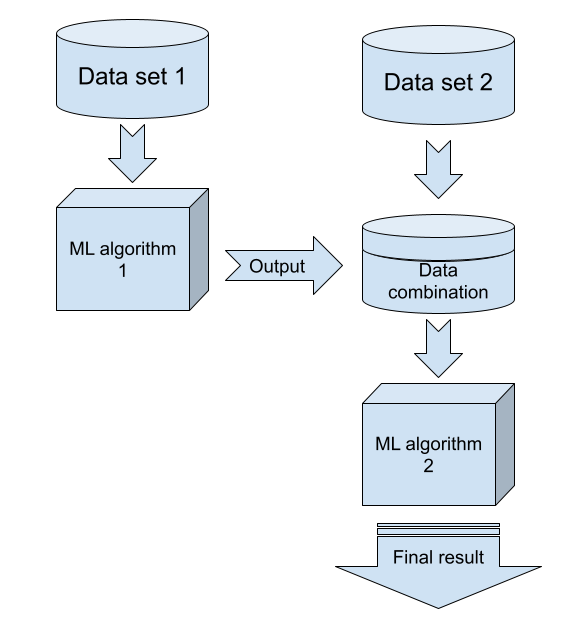
\includegraphics[width=0.5\textwidth,]{./appendices/hybrid-ml-model}
    \caption{Simplistic example of a hybrid machine learning model.
    The first algorithm learns from the initial data,
        and the results are used with a second data set to train another algorithm.
        \label{fig:hybrid-ml-model}}
\end{figure}

It is not feasible to use anomaly detection on its own to estimate ticket amounts
as plain sum of anomalies detected
is not correlating with tickets received.
Using pure statistical values of the log data
such as log rows per day
would possibly give some results with a single algorithm,
but only if the amount of log events correlates strongly with tickets received.
We can, however,
amplify our ticket estimating algorithm with anomaly feature values.
As we first count the anomaly numbers with the anomaly detection algorithm
and use the statistical features of the results in another algorithm,
like regression algorithm,
we get more relative information to use
when creating the final ticket number estimations.
This is explained in more detail
later in section~\ref{subsec:pipe-random-delay-and-timeframe-compression}.


%% ************************************************************************************************************


\subsection{HML phase 1: PCA-based anomaly detection}\label{subsec:pipe-pca-ada-input-output}


%% ............................................................................................................

\subsubsection*{PCA-ADA input feature formatting}
In Azure ML Studio, the only selectable module for
anomaly detection is the PCA-based anomaly detection
algorithm (PCA-ADA), which is explained in section~\ref{subsec:bg-pca-ada}.
However,
with textual input like logs
it can be used in at least two ways.

First,
input data can be fed to
the algorithm trainer as is,
letting the PCA-ADA component
do the work without further modifying the log rows.
This way,
the component tries to recognize the anomalies
based on all the information included in the row.
Practically this means,
that the component processes data in textual format
making each row in the input
a feature as a whole to consider.
As we discussed in the section~\ref{subsec:meth-data-anonymization},
unique values should be removed from the log rows
and the data should be somewhat clean.
PCA should be able to find similar values
and create anomaly score with purely textual features.
However,
it is probable that with a single word change on a message feature,
PCA defines two rows as completely different.

Second option is to convert the textual features into numerical features.
This can be done
either with the "Extract N-Gram Features from Text" component,
or the "Feature Hashing" component which uses n-gram feature extraction behind the scenes.
With n-gram feature extracting,
as explained in the section~\ref{subsec:bg-ngram-features-and-hashing},
each word or n-gram is converted to a number of said instance found on the row being processed,
and each row can be presented as a sequence of numbers
indicating the number of those features.

An N-gram feature can in addition have a weight
based on the frequency the n-grams appear
in the entire data.
Different weights usable in Azure ML component
are listed in table~\ref{tab:n-gram-weights}.
During this study,
only binary weight was used,
so it is possible that improved results could have been acquired with a different weight method.

\begin{table}[htb]
    \begin{tabularx}{\textwidth}{|L{0.25\textwidth}|X|}
        \hline
        \textbf{N-gram weight}  & \textbf{Explanation}       \\ \hline
        Binary Weight       & Assigns a binary presence value to the extracted n-grams. The value for each n-gram is 1 when it exists in the document, and 0 otherwise.     \\ \hline
        TF Weight           & Assigns a term frequency (TF) score to the extracted n-grams. The value for each n-gram is its occurrence frequency in the document.                \\ \hline
        IDF Weight          & Assigns an inverse document frequency (IDF) score to the extracted n-grams. The value for each n-gram is the log of corpus size divided by its occurrence frequency in the whole corpus. \verb-IDF = log of corpus_size / document_frequency-        \\ \hline
        TF-IDF Weight       & Assigns a term frequency/inverse document frequency (TF/IDF) score to the extracted n-grams. The value for each n-gram is its TF score multiplied by its IDF score.      \\ \hline
    \end{tabularx}
    \caption{Statistic metrics of the time frame compression that are considered possibly useful for ML algorithm.~\cite{azure2021ngramfeature}}
    \label{tab:n-gram-weights}
\end{table}

As stated,
a vast dictionary of n-grams demands resources from the ML computing instances
as every new n-gram in the dictionary adds another column to the training dataset.
To reduce the amount of memory needed,
the "Feature Hashing" component can be used.
By hashing the n-gram features,
the amount of resources needed by the pipeline
can be significantly reduced.
Feature hashing allows us to use the entire amount of data as an input
if feature hashing parameters are tuned enough.
However,
as discussed in the section~\ref{subsec:bg-ngram-features-and-hashing},
the greater the compression is,
the more information is lost
to reduce the need for resources.

Before the n-gram operations,
the textual data can be preformatted in Azure ML Studio
with "Preprocess text" -component.
This component includes several options to choose from
in order to clean text to more processable form.
Most useful options to select from are
\textit{stop word removal} (which removes uninformative words such as "the", "is" and "and"),
\textit{lemmatization} (which converts words to their canonical form,
for example "bigger mice eating" to "big mouse eat"),
\textit{detect sentence} (which inserts a sentence boundary symbol
to help algorithm text analysis),
\textit{text case normalization} (which normalizes all characters to lower case
to reduce the number of different words when first letter is capitalized),
and various \textit{character removals} (which range from number, special character, and duplicate character,
to url and email address removal possibilities).
Text preprocessing usually helps to reduce the number of features
when text is used in n-gram feature extraction and feature hashing.
Most of the options, however,
do not work well with other languages than English,
which might create issues with this study case
as logs contain a mixed amount of English and Finnish words.~\cite{azure2021preprocess}

In the end,
the need for memory proved problematic
and pure n-gram feature extracting forced us
to reduce the data size to only 2\%
in order to finish the algorithm training pipeline.
This amount was considered to be too low
for reliable algorithm training results.
Still,
all variations of input feature formatting were tested
to see how much possible shortcomings would affect the results.
More about the memory issue is discussed
in the section~\ref{subsec:res-memory-issues}.


%% ************************************************************************************************************


\subsubsection*{PCA output and anomaly probability}

The output values of the PCA-ADA component,
as explained in the section~\ref{subsec:bg-pca-ada},
are normalized so the values range between 0 and 1.
This anomaly probability value
is the main output of hybrid ML phase 1.
Based on our initial hypothesis,
that each anomalous event in the log
is linked to a real life support ticket received,
the bigger a single anomaly probability value is for a log row,
the more likely is that the row is related to a ticket inducing event.
Further processing steps of the output values
are discussed later in the section~\ref{subsec:pipe-random-delay-and-timeframe-compression}.

%% ************************************************************************************************************


\subsubsection*{Unconventional training approach}\label{subsec:pipe-unconventional-training}

As stated in section~\ref{subsec:bg-machine-learning},
the approach we attempt in this study is,
if expression is allowed, unorthodox.
Typically,
the data points used in ML algorithm training and validating
should always be different.
Acting otherwise leads to algorithm processing with
same data it was trained with,
thus creating a situation
where algorithm already knows what to do with the current data point.
If the results were validated after this
the algorithm would get an unreliably good score
as it had the validation data already in the training phase.
This could be compared to
giving some right answers to students during a test
and scoring test results as if no help was given.
However,
due to the nature of the study problem and contents of the data,
it was decided to test whether bending this rule
would provide better results in algorithm training.

The large amount of data was enough
to cause issues with memory.
Although this problem was succesfully circumvented,
the hybrid approach and the time frame compression
(discussed later in section~\ref{subsec:pipe-random-delay-and-timeframe-compression})
resulted in a significant data loss in phase 2.
As a general rule of thumb in ML training,
only 20--30\% of the data is used to validate the algorithm.
With the hybrid ML approach,
the validation results in phase 1
are what actually form the data used in phase 2.
This data is further compressed to time frame groups
leading to only a few dozen data points in phase 2 ML training
compared to millions of rows in phase 1.

Because of the way the PCA-based anomaly detection algorithm works,
the over-lapping data points are not as big of an issue
as it would be with other types of algorithms
like regression algorithms.
This is why we could use part of the data
for training the anomaly detection algorithm as usual
and then use all the data available for validation
without overfitting the algorithm,
which happens when algorithm fits to the training data well,
but cannot generalize with new data~\cite{wang2016machine}.
Also, because the main forecasting functionality comes in the phase 2,
overfitting in phase 1 may not cause issues.

To verify if this unconventional training method gives good results without issues,
the trained algorithms were tested with new production data
that had zero overlapping data points with training and validation data.
This training method was also compared to a traditionally trained algorithm
to see the differences in results of both training styles.
This way we were able to compare different training approaches
to determine the best overall pipeline structure.

Kind of informal mention considering
the traditional training approach in our study case
is the data splitting of the log data for algorithm training.
Because of the hybrid model,
and the data consisting of log rows,
we cannot make a random split for the training and validation data
as is usually done.
Purely for training
the random splitting can be done,
but if data in phase 1 is split randomly for validation,
some anomalous rows could be skipped from a time frame
that would be crucial information for the estimations in phase 2.
This is why we must make sure the possible data splitting for validation data
is chronological in phase 1.


%% ************************************************************************************************************


\subsection{HML phase 2: Ticket count estimation with regression}\label{subsec:pipe-regression-estimating}


%% ............................................................................................................

\subsubsection*{Input data random delay and time frame compression}\label{subsec:pipe-random-delay-and-timeframe-compression}

As mentioned previously in section~\ref{sec:introduction},
it takes time for a bank clerk to notice the error in the RPA process,
send a technical support ticket considering the issue,
and for the support team to redirect the request to the corresponding developer team.
As several steps of human interaction and workday schedules
are in between the event of logging and ticket receiving,
the random delay of such may span from hours to days.
Random delay in input data features
is not an unusual aspect in time-series forecasting.
Time-series in the context of ML
refers to data features that vary over time
and can be affected by past values.~\cite{palma2016time}
As an example,
an ML algorithm could try to predict future weather
based on measured temperature and air pressure.
Both these features change over time
and also affect their own future values.

This study, however,
is not about time-series
because the majority of the log rows
are not affected by previously logged events.
As random delay of such
does not seem to be trivial to take into account
with ML algorithms,
a simple method to solve this was used
where log rows were grouped by time stamp
into certain time frame groups.
We call this method "time frame compression method".

Time frame compression means,
that in order to eliminate the effects of random delay
we compress some features into a certain time frame
at least as long as the longest estimated delay.
Simply put,
if we count possible anomalies during one hour of log,
we cannot compare this number to actual tickets received
at the same hour or the next.
What we can do,
with time frame compression,
is that we count some statistical values of anomaly estimates,
for example, the mean and median values of a week,
and then compare these numbers with the tickets received
during the same week.
Statistically important and thus compressible features of a time frame
were determined to be the log row count,
amount of unique job IDs, and anomaly probability metrics.

The amount of log rows describes
how many logged issues occurred in a time frame.
Alone,
this feature may not give much insight
as the amount of logs is possibly not linearly comparable
to the amount of tickets received.
Combined to other statistical metrics
it may, however,
provide additional value for ticket forecasting.
Job ID is the identification information of a specific RPA automation execution run.
It means,
that the job ID is not unique for each log row,
but it binds together all the log entries on the same RPA automation execution.
By counting the amount of unique job IDs in a time frame
we can get insight about the amount of automation jobs executed during the time frame.
This metric is important with the total row count:
low number of unique jobs with high number of total rows
indicates that plenty of loggable events and possible errors happened during the time frame,
whereas high number of unique jobs combined to low number of rows
imply that not much happened (or perhaps executions were completely crashed).

By the original hypothesis,
anomalies in the logs are linked closely to the support tickets received.
The anomaly detection algorithm produces a probability value of
how strongly a row is considered to be an anomaly,
thus,
the mean and median values of the anomaly probabilities in a time frame
indicate how anomalous all the executions within a time frame have statistically been.
However,
when compressing the anomaly probability metrics in a time frame,
some information is bound to be lost.
The mean and median values do not provide information
about the anomaly probability value distribution.
There may be few very high values and a lot of low probabilities,
and it would lead to the same mean value
as if there were a lot of slightly higher probabilities and just few very low values.
By adding more statistical values
we can reduce the loss of information caused by time frame compression.
If the original hypothesis is correct,
the most relevant anomaly values are the highest anomaly probabilities.
Thus,
calculating higher quantiles and the amount of values exceeding them
should improve the estimation abilities of the algorithm.

\begin{table}[htb]
    \begin{tabularx}{\textwidth}{|L{0.4\textwidth}|X|}
        \hline
        \textbf{Statistic feature}  & \textbf{Explanation (in time frame)}       \\ \hline
        LogRowCount              & Number of rows/instances overall           \\ \hline
        UniqueJobIDs             & Amount of unique job IDs                   \\ \hline
        AnomalyProbabilityMean   & Mean value of anomaly probabilities        \\ \hline
        AnomalyProbabilityMedian & Median value of anomaly probabilities      \\ \hline
        AnomalyQuantile90        & 90-quantile value of anomaly probabilities \\ \hline
        AnomalyCountOverQ90 & Number of instances with anomaly probability over 90-quantile \\ \hline
    \end{tabularx}
    \caption{Statistic metrics of the time frame compression that are considered possibly useful for ML algorithm.}
    \label{tab:statistic-features}
\end{table}

In table~\ref{tab:statistic-features},
all the statistic metrics considered interesting and valuable
from time frame compression of the log rows
are listed with short explanation.
In the pipeline,
the statistical values are calculated
using the R-script executing component.
An example of such script executed by the "Execute R Script" component
is presented in appendix~\ref{sec:app-r-script}.

The result values of the anomaly detection algorithm
are time-frame-compressed along with the technical ticket timestamps,
which form the second part of our data.
The timestamp data, however,
is compressed simply into a count of tickets received in the defined time frame.
Now we have a comparable feature
that is usable by regression algorithms.


%% ************************************************************************************************************


\subsubsection*{Regression algorithm options}\label{subsec:pipe-regression-algorithm-options}

Azure ML Studio has six usable regression algorithms.
One of them,
Fast Forest Quantile Regression,
is used to explain the distribution of the value being predicted.\cite{azure2021fastforestquantile}
In our case, however,
this does not provide any use for us
as we are predicting the ticket count per time frame.
The distribution of tickets within each time frame is irrelevant.

The remaining five algorithms are presented below:
\begin{enumerate}
    \item Linear regression~\cite{azure2021linear}
    \item Boosted decision tree regression~\cite{azure2022boosteddecisiontree}
    \item Decision forest regression~\cite{azure2021decisionforest}
    \item Neural network regression~\cite{azure2021neuralnetwork}
    \item Poisson regression~\cite{azure2021poisson}
\end{enumerate}

Linear regression is the simplest of the algorithms,
and even though it can be easily explained with the least square principle
described in section~\ref{subsec:bg-regression-ml},
the linear regression component is capable of more advanced methods,
such as gradient descent.
Poisson regression works only for Poisson distributed data.
As the distribution of the anomalies or ticket inducing log events is not certain,
we cannot rule this method out before seeing the results.

The other components with \textit{tree} or \textit{forest} in their name
are based on the same algorithm model called \textit{decision trees}.
Decision trees are models
which run a series of simple tests
for all data points in each branching node.
The data is moved on like water along the tree from trunk to branches
until it reaches the leaf node which marks the decision-making point.
When multiple trees are placed in a series,
the decision tree becomes a forest.~\cite{azure2021decisionforest}

Neural network mimics the way the human brain operates.
Multiple layers of neurons form a network,
where data is passed to the next node for further processing.
Unlike with decision tree nodes,
neurons in neural network do not form separate branches,
but each node can be reached via multiple paths.~\cite{mahesh2020machine}

All of these regression algorithm models
were tested and their results validated with new data
in order to find the one with the most promising results.


%% ************************************************************************************************************

\subsection{Pipeline branching}\label{subsec:pipe-branching}

In order to find the best possible combination of components,
all different combinations must be compared.
As the pipeline is structured in a tree-like flow,
each node that includes more than one possible choice
diverges the pipeline into branches.
Several diverging points have been mentioned before in this study,
and in this section we join the information together.

First,
the error message used to calculate the anomaly probability of a log row
had two options.
We could either use simple \textit{message},
or more verbose \textit{rawmessage}.
This textual data could be fed to the ADA-component in several forms.
Most straightforward way was using textual data without any preformatting or modification.
Text could also be run through the "Preprocess text" -component.
N-gram features could have been extracted from the original or the preprocessed text
and these features could have been used instead.
Instead of n-gram features,
the textual data could be converted to numeric
also with the "Feature Hashing" -component.

After getting the ADA-component results,
phase 1 is finished.
At the beginning of the next phase,
the anomaly probabilities were compressed with R-code or SQL query.\@
In this phase,
branching of the pipeline was due to
comparing results without the anomaly probability values calculated in phase 1,
and then utilizing different regression algorithms in phase 2.
In practice this means
that in order to validate the results against our initial hypothesis,
we used pure statistical log data,
such as row count and unique job ID count
without anomaly probabilities,
to determine whether anomaly metrics provided any insight regarding the ticket data.
When using n-gram features or hashed features,
these additional column features were also included for this comparison,
as forming them does not depend on the anomaly properties of the log instance.

Each branching step, or layer,
multiplies the amount of comparable values used in final comparison
that would determine the best possible pipeline combination.
These layers are simplified in table~\ref{tab:ml-pipeline-branching}.

\begin{table}[htb]
    \centering
    \begin{tabularx}{\textwidth}{|L{0.3\textwidth}|L{0.45\textwidth}|X|}
        \hline
        \textbf{Branching node}           &
        \textbf{Options}                 &
        \textbf{Divergent count} \\ \hline
        Input text column                  & \begin{tabular}[c]{@{}l@{}}message \\ rawmessage\end{tabular}                 & 2                        \\ \hline
        Text preprocess                    & \begin{tabular}[c]{@{}l@{}}Yes\\ No\end{tabular}                              & 2                        \\ \hline
        Numeric conversion                 & \begin{tabular}[c]{@{}l@{}}No\\ N-gram Feature\\ Feature Hashing\end{tabular} & 3                        \\ \hline
        ADA training                       & \begin{tabular}[c]{@{}l@{}}Unconventional \\ Proper\end{tabular}              & 2                        \\ \hline
        Validation without anomaly metrics & \begin{tabular}[c]{@{}l@{}}Yes\\ No\end{tabular}                           & 2                        \\ \hline
        Regression algorithms &
        \begin{tabular}[c]{@{}l@{}}
            Linear regression\\
            Boosted decision tree regression \\
            Decision forest regression \\
            Neural Network Regression \\
            Poisson regression \\
            \end{tabular}
        &   5 \\ \hline
    \end{tabularx}
    \caption{Pipeline divergent layers}
    \label{tab:ml-pipeline-branching}
\end{table}

The divergent count implies the number of branches
diverging from the previous component.
The total count of branch ends, or leaves,
would then be the multiplication of all divergent counts,
totaling to 240 comparable pipeline combinations.
Moreover,
n-gram feature extraction and feature hashing
have several tunable parameters
that strongly influence the end results of the algorithm training.
To reduce this amount when considering the best possible pipeline,
we simplified this by narrowing down the options
based on initial test run results of some of the divergent options.

For example,
n-gram feature component suffered greatly from the memory problem
(which we discuss more in section~\ref{subsec:res-memory-issues}),
and the data amount that the "Extract N-Gram Features from Text" -component was able to handle
comprised of only 2\% of the original data.
This was deemed as too small of an amount for training an ML algorithm
as it is extremely likely that with 98\% of the data skipped,
some possibly relevant rows for the ticket anomalies would also get trimmed out.

The flowchart of pipeline with branching options visualized
is illustrated in figure~\ref{fig:pipeline-flowchart}.
The final pipeline structure used for result acquiring
can be seen in the appendix~\ref{sec:app-final-pipeline-structure}.
\begin{figure}[htb]
    \centering
    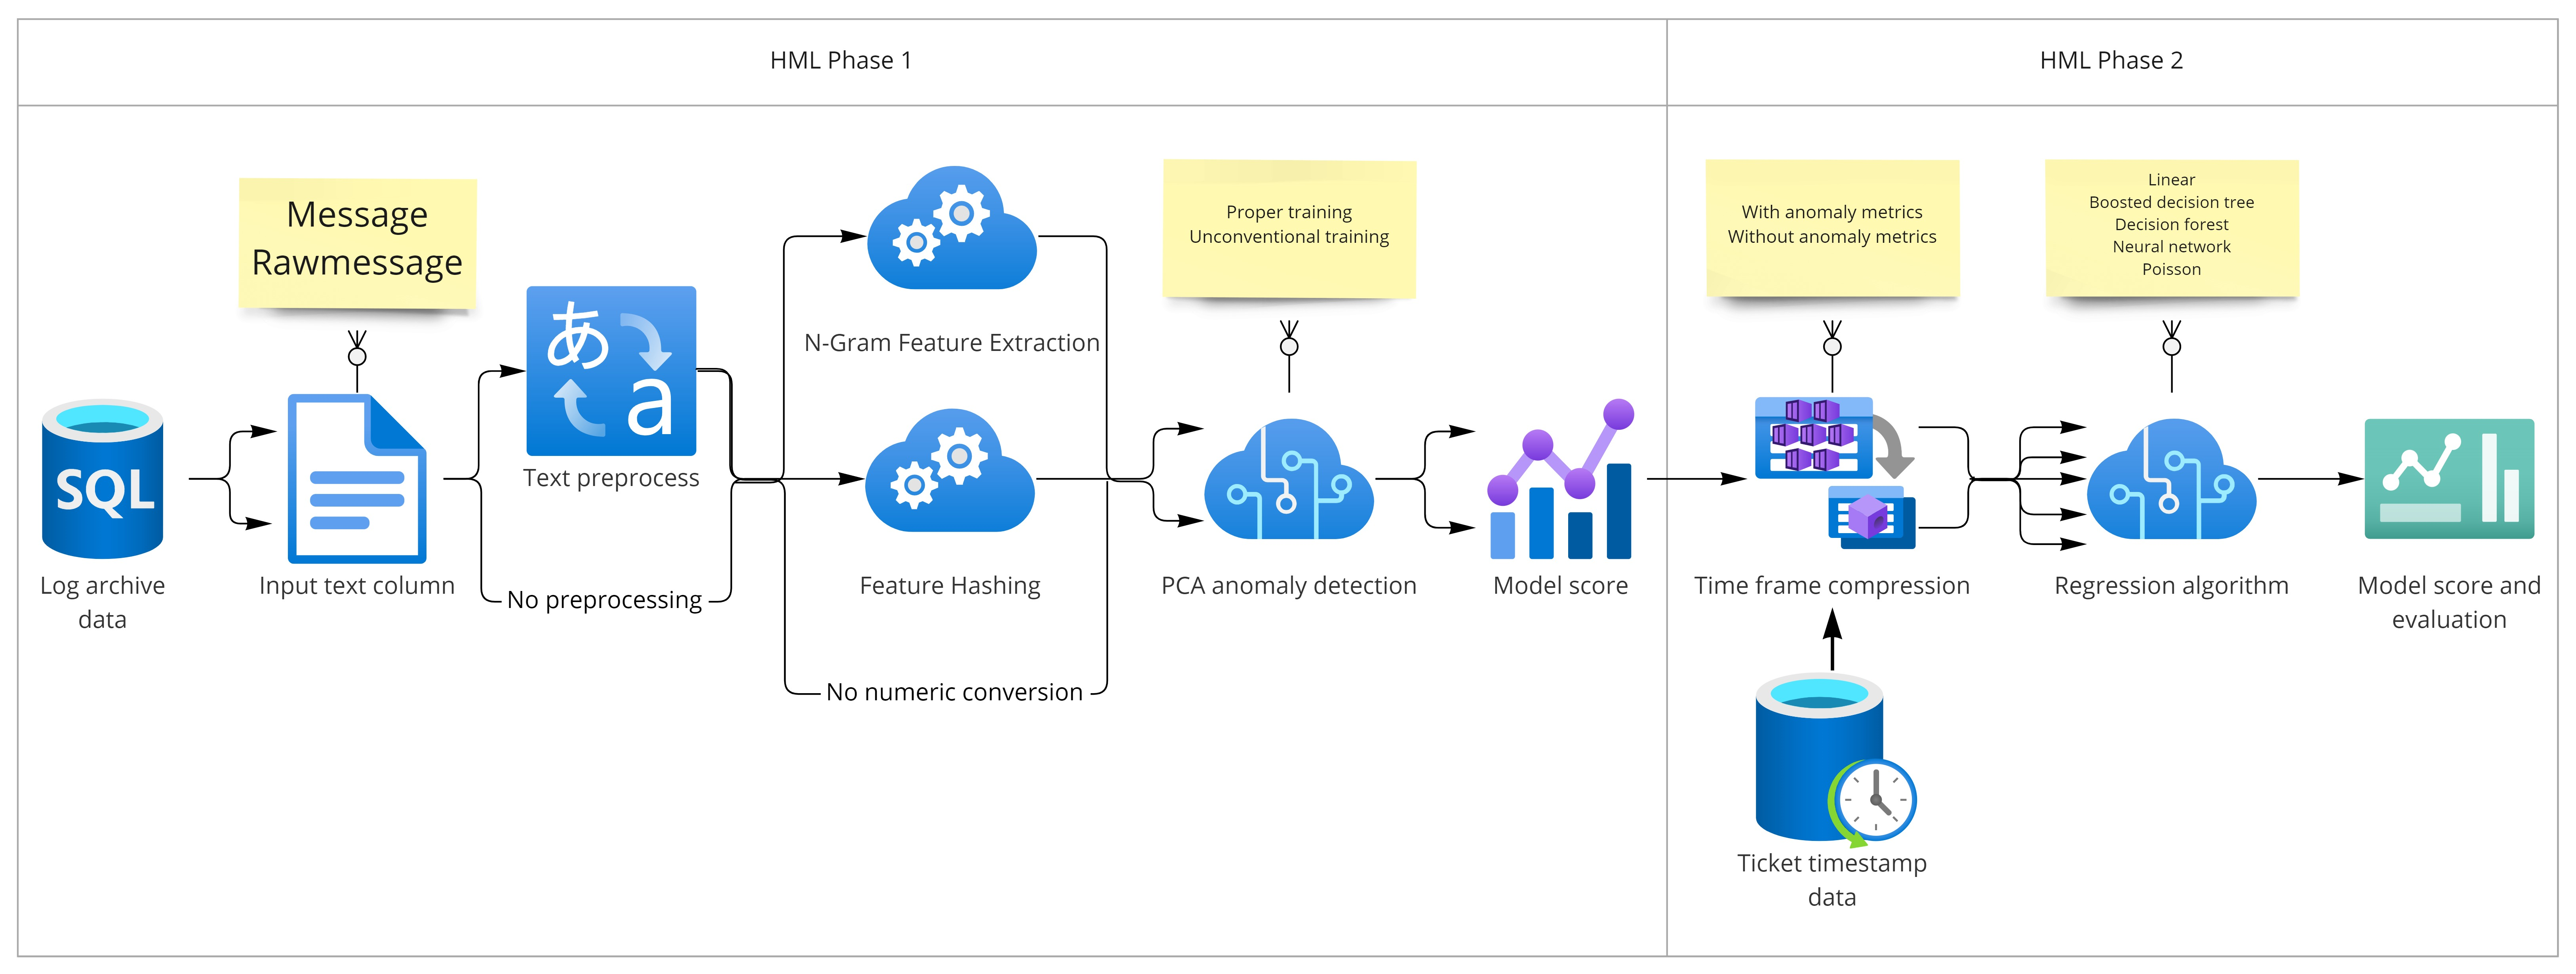
\includegraphics[width=\textwidth]{./appendices/pipeline-flowchart.jpg}
    \caption{Pipeline flowchart with branching steps illustrated.
    HML phase boundaries are made visible for clarity.
    \label{fig:pipeline-flowchart}}
\end{figure}


%% ************************************************************************************************************


\subsection{Comparable metrics}\label{subsec:pipe-comparable-metrics}

In previous sections we have discussed different approaches that could be used
to get the best results from the ML training.
In order to find the best possible combination of components,
we must compare different results,
and for this we need comparable metrics.
After training,
the Azure regression algorithms are scored with validation data.
The final output from this is a numeric \textit{Scored Labels} feature.
In our study case,
this value is what the algorithm estimates the ticket count on the time frame to be.
Next,
the "Evaluate Model" -component calculates a few evaluation metrics
to be used for result comparison.
These metrics for regression algorithm are listed
in table~\ref{tab:comparable-metrics}.

\setlength{\tabcolsep}{5pt}
\begin{table}[htb]
    \begin{tabularx}{\textwidth}{|L{0.35\textwidth}|X|}
        \hline
        \textbf{Name of the metric}             & \textbf{Explanation}  \\ \hline
        Mean Absolute Error (MAE)               & Measures how close the predictions are to the actual outcomes;
            thus, a lower score is better. \\ \hline
        Root Mean Squared Error (RMSE)          & Creates a single value that summarizes the error in the model.
            By squaring the difference, the metric disregards the difference between over-prediction and under-prediction. \\ \hline
        Relative Squared Error (RSE)            & Normalizes the total squared error of the predicted values
            by dividing by the total squared error of the actual values. \\ \hline
        Relative Absolute Error (RAE)           & The relative absolute difference between expected and actual values;
            relative because the mean difference is divided by the arithmetic mean. \\ \hline
        Coefficient of Determination (CoD)      & Often referred to as $R^{2}$,
            represents the predictive power of the model as a value between 0 and 1.
            Zero means the model is random (explains nothing);
            1 means there is a perfect fit.
            However, caution should be used in interpreting $R^{2}$ values,
            as low values can be entirely normal and high values can be suspect. \\ \hline
    \end{tabularx}
    \caption{Comparable metrics provided by "Evaluate Model" component for regression algorithm.\cite{azure2021evaluate}}
    \label{tab:comparable-metrics}
\end{table}

Our goal is to find a connection
between the log anomalies and the ticket time\-stamps.
Our initial hypothesis suggested
that the most anomalous events in the logs
would be more related to the ticket events than other rows.
By this logic,
we compared the algorithm evaluation metrics
with the metrics produced by the neighboring pipeline branch
where anomaly probabilities had been removed.
The best algorithm should be found in a branch
where the evaluation values are significantly better
than the neighboring branch from which the anomaly values have been removed.
This proves, that the anomaly probability values improve the algorithm estimations,
which indicates that the hybrid algorithm combination has indeed found the connection
between anomalies and ticket timestamps.
This will also be our logical basis when selecting certain algorithms for further tests.



\clearpage
%!TEX root = thesis.tex
%% %% ***************** Results *****************


\section{Results}\label{sec:results}


\subsection{Azure and Azure ML Studio}\label{subsec:azure-and-azure-ml-studio}

<general about ml inside azure>

\subsubsection*{Azure resources}

<what resources was needed inside Azure?>

<virtual machines etc.>




\subsubsection*{Azure ML Studio components}
<clusters and data>

<Memory problems>

During the initial pipeline runs
the execution came to an abrupt stop
and Azure notified about memory issues.
These problems were linked to the data amount
which had to be reduced to 600 megabytes
before any pipeline could be finished using the data.
This reduction was against the initial goal
where preferably all the data could have been used.

Considerable amount of time was used
to fix or avoid this issue
but nothing clear was found
that would explain the error received.
While working with the issue
it was also noted
that data needed more cleaning
in order to ease the preprocessing phase
as described with more detail in section~\ref{subsec:rmm-data-anonymization}
Thus,
the data had to be imported from log archive
and anonymized once more.

Two choices was possible to take:
\begin{enumerate}
    \item Continue working with full data
    and attempting to fix the memory issue
    by consulting Azure experts
    \item  Trim the data to reduce the data size
    by declaring info-type log messages
    as unnecessary
    and working with vastly diminished data
    until the memory issue would be solved
    one way or another
\end{enumerate}

To advance the study more efficiently
it was decided to trim info-type log messages from data
hence reducing the data amount considerably.
Meanwhile,
<fixing the memory issue>

\subsection{ML training and validation}\label{subsec:ml-training-and-validation}

<anomaly detection>

<N-Gram Feature extracting>

<Some regression algorithm to predict event count.
Poisson only for poisson distributed data.>

<two-class classification>
<support vector machine etc>

preformatting data! \\
\begin{enumerate}
    \item remove fingerprint etc unique values from raw message
    \item calculate anomaly probability per line
    \item [!] CAN WE COMBINE THIS PER JOB-ID?
    \item create new table consisting:
    \begin{enumerate}
        \item amount of rows per timeframe
        \item amount of unique job ID's per said timeframe
        \item anomaly probability value (median, mean etc)
        \item efecte tickets received in said timeframe
    \end{enumerate}
\end{enumerate}

\subsubsection*{<Integrating with timestamps>}
To avoid the problem with random delays
between log rows and technical ticket timestamps,
log rows were grouped by time stamp
certain time frame groups.

%% using verbatim to avoid douple line breaks for pdf readability
\begin{verbatim}
  <todo:

  ***A***
  count sum of incidents in timeframe x
  set x to each row in data by timestamp
  predict amount of incidents based on data

  ***B***
  Use efecte data as reference values
  (regression, predict amount in timeframe -> compare)
  (classification, count TRUE in timeframe -> compare amount)

  >
\end{verbatim}


%% TODO: TEST WITHOUT ANOMALY PROBABILITY METRICS!!!
%% ie. is the anomaly phase of the hybrid learning really usefull
%% Do log row amount and jobid amount correlate more to tickets as features?




\clearpage
%!TEX root = thesis.tex
%% %% ***************** Summary *****************

\section{Summary}\label{sec:summary}
\todo{Very under construction...}

<Sum up here what we did and why>

\subsection{Discussion}\label{subsec:discussion}
<Here some thinking what should have been improved>

Integrating with real time logging?

\subsubsection*{Data formatting}
The most time-consuming tasks in the study
was without a doubt
the anonymization and preformatting of the data.
Although sensitive information may sometimes be crucial in error fixing
as problems may consider just one client,
it is necessary that the data sanitation is possible to do
in order to use the data in less secure environment.
By preformatting the data in such way
that all different personal information types
do not differ between use cases.
%% TODO: hetu in weird form


\subsubsection*{Possible ML methods}
Some sort of time delay forecasting?\cite{erharter2021pointlessness}
Could we estimate the number of tickets
based on some log metrics in time frame?

Memory error fixing would have given more options.

\todo{Something else specifically needed?}

If log would have been better organized/preformatted
it would have been possible to use One-Class Support Vector Machine.
This, however,
would have needed a manually constructed dataset
including only "normal" log events
or such events that could have been certain of
that they were not part of the ticket inducing issues.

%% TODO: Shifting timeframes from mon-sun -> sat-fri ?!?!
\todo{Shifting timeframes from mon-sun -> sat-fri }

Some more testing would be needed to determine
whether splitting data randomly or not in the phase 1
provides better results.
By splitting data randomly
it is possible to miss important anomalous rows that come in groups
which would provide necessary insight to identify anomalous events.

%% TODO:
\todo{Show some explaining graphics, here or elsewhere.}


The original hypothesis was
that anomalous events in the logs
were clearly linked to the tickets received.
However,
as memory errors due to the size of data forced us to skip info-typed rows,
it is possible the data anomalies did not reflect to the tickets.
As stated before,
multiple error lines in the log may be linked to a single issue,
which could make the ticket inducing events
more common log feature.
Thus,
by tuning the statistical values used
to take into account more common error messages,
it could have been possible to get better results.

%% TODO:
\todo{Could anomaly probability metrics be calculated per job ID?}


\clearpage


%% Lähdeluettelo
\thesisbibliography
\bibliographystyle{IEEEtran}
\bibliography{refs}
%%


%% Appendices
%!TEX root = thesis.tex
%% %% ***************** Appendices *****************

\clearpage


\thesisappendix

\section{Final pipeline structure}\label{sec:app-final-pipeline-structure}

\begin{figure}[htb]
    \centering
    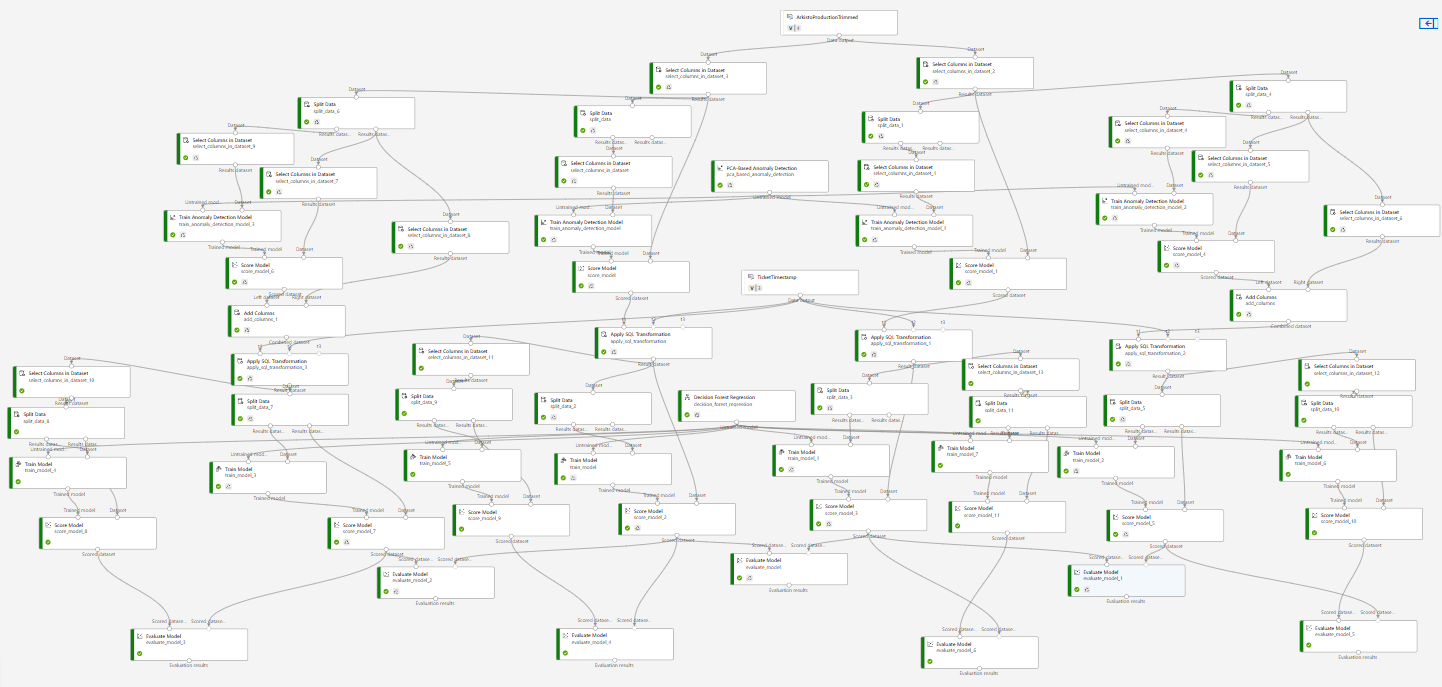
\includegraphics[width=180mm,angle=90]{./appendices/pipeline-draft}
    \caption{Final pipeline structure.
    It includes message and rawmessage branches, their pure, preprocessed and feature hashing combinations,
    two algorithm comparison blocks, and a three final test branches using fresh data for for model scoring.
    \label{fig:app-pipeline-structure}}
\end{figure}

\clearpage

%% ************************************************************************************************************

\section{RPA log data example 1}\label{sec:app-log-data-input}

RPA log data in raw format after anonymizing and exporting to local environment.
Here are four lines of log events with different log levels,
first line being a header row.
First example has been reduced in size with \verb-[...]--marking.
Data is in CSV-format,
with each column separated by comma.
The rawmessage is injected inside CSV
in JSON-format.

This data was fetched from the SQL-database
with the following SQL-script:
\verb=SELECT OrganizationUnitId,TenantId,TimeStamp,Level,=

\verb=ProcessName,JobKey,RobotName,Message,RawMessage,=

\verb=MachineId FROM [dbo].[logs]=

\begin{Verbatim}[fontsize=\tiny]
"OrganizationUnitId","TenantId","TimeStamp","Level","ProcessName","JobKey","RobotName","Message","RawMessage","MachineId"
"5","5","1/2/2020 12:55:24 PM","4","rpa-bank-020-lainahakemuksien-tietojen-siirto_Samlink Production",
    "b03cfd05-1807-45e7-b962-c9d95e49a3fc","RPA-RPP-4","System.IO.IOException: The process cannot access the file
    'W:\RPA\BANK\020 lainahakemuksien tietojen siirto\prod\Config.xlsx' because it is being used by another process.
    at System.IO.__Error.WinIOError(Int32 errorCode, String maybeFullPath)
    at System.IO.FileStream.Init(String path, FileMode mode, FileAccess access, Int32 rights, Boolean useRights,
        FileShare share, Int32 bufferSize, FileOptions options, SECURITY_ATTRIBUTES secAttrs, String msgPath, Boolean
        bFromProxy, Boolean useLongPath, Boolean checkHost)
    at System.IO.FileStream..ctor(String path, FileMode mode, FileAccess access, FileShare share, Int32 bufferSize,
        FileOptions options, String msgPath, Boolean bFromProxy)
    at System.IO.FileStream..ctor(String path, FileMode mode, FileAccess access, FileShare share, Int32 bufferSize,
        Boolean useAsync)
        [...]
    at System.Activities.Runtime.ActivityExecutor.ExecuteActivityWorkItem.ExecuteBody(ActivityExecutor executor,
        BookmarkManager bookmarkManager, Location resultLocation)","{
    "message": "System.IO.IOException: The process cannot access the file 'W:\\RPA\\BANK\\020 lainahakemuksien tietojen
        siirto\\prod\\Config.xlsx' because it is being used by another process.\r\n   at System.IO.__Error.WinIOError
        (Int32 errorCode, String maybeFullPath)\r\n   at System.IO.FileStream.Init(String path, FileMode mode,
        FileAccess access, Int32 rights, Boolean useRights, FileShare share, Int32 bufferSize, FileOptions options,
        SECURITY_ATTRIBUTES secAttrs, String msgPath, Boolean bFromProxy, Boolean useLongPath, Boolean checkHost)\r\n
        at System.IO.FileStream..ctor(String path, FileMode mode, FileAccess access, FileShare share, Int32 bufferSize,
        FileOptions options, String msgPath, Boolean bFromProxy)\r\n   at System.IO.FileStream..ctor(String path,
        FileMode mode, FileAccess access, FileShare share, Int32 bufferSize, Boolean useAsync) [...]   at
        System.Activities.Runtime.ActivityExecutor.ExecuteActivityWorkItem.ExecuteBody(ActivityExecutor executor,
        BookmarkManager bookmarkManager, Location resultLocation)",
    "level": "Error",
    "logType": "User",
    "timeStamp": "2020-01-02T14:55:24.6280687+02:00",
    "fingerprint": "5ebb011b-fb3d-402a-8024-79a21e6629c9",
    "windowsIdentity": "LOCAL\\WinID",
    "machineName": "T4690A3018",
    "processName": "rpa-bank-020-lainahakemuksien-tietojen-siirto_Samlink Production",
    "processVersion": "1.0.7244.25507",
    "jobId": "b03cfd05-1807-45e7-b962-c9d95e49a3fc",
    "robotName": "RPA-RPP-4",
    "machineId": 28,
    "fileName": "GlobalHandler"
}","28"
"5","5","1/2/2020 12:55:24 PM","0","rpa-bank-020-lainahakemuksien-tietojen-siirto_Samlink Production",
    "b03cfd05-1807-45e7-b962-c9d95e49a3fc","RPA-RPP-4","Log Error Executing","{
    "message": "Log Error Executing",
    "level": "Verbose",
    "logType": "Default",
    "timeStamp": "2020-01-02T14:55:24.6280687+02:00",
    "fingerprint": "3c68aacf-dd4c-4ad4-8045-043e72b35bb7",
    "windowsIdentity": "LOCAL\\WinID",
    "machineName": "T4690A3018",
    "processName": "rpa-bank-020-lainahakemuksien-tietojen-siirto_Samlink Production",
    "processVersion": "1.0.7244.25507",
    "jobId": "b03cfd05-1807-45e7-b962-c9d95e49a3fc",
    "robotName": "RPA-RPP-4",
    "machineId": 28,
    "fileName": "GlobalHandler",
    "activityInfo": {
        "Activity": "UiPath.Core.Activities.LogMessage",
        "DisplayName": "Log Error",
        "State": "Executing",
        "Variables": {
            "answer": "",
            "retry": "0",
            "HetuFound": "False",
            "FilteredException": ""
        },
        "Arguments": {
            "Message": "System.IO.IOException: The process cannot access the file 'W:\\RPA\\BANK\\020 lainahakemuksien
                tietojen siirto\\prod\\Config.xlsx' because it is being used by another process.\r\n   at System.IO.
                __Error.WinIOError(Int32 errorCode, String maybeFullPath)\r\n   at System.IO.FileStream.Init(String
                path, FileMode mode, FileAccess access, Int32 rights, Boolean useRights, FileShare share, Int32
                bufferSize, FileOptions options, SECURITY_ATTRIBUTES secAttrs, String msgPath, Boolean bFromProxy,
                Boolean useLongPath, Boolean checkHost)\r\n   at System.IO.FileStream..ctor(String path, FileMode mode,
                FileAccess access, FileShare share, Int32 bufferSize, FileOptions options, String msgPath, Boolean
                bFromProxy)\r\n   at System.IO.FileStream..ctor(String path, FileMode mode, FileAccess access, FileShare
                share, Int32 bufferSize, Boolean useAsync)\r\n   at MS.Internal.IO.Zip.ZipArchive.OpenOnFile(String
                path, FileMode mode, FileAccess access, FileShare share, Boolean streaming)\r\n   at System.IO.
                Packaging.ZipPackage..ctor(String path, FileMode mode, FileAccess access, FileShare share, Boolean
                streaming)\r\n   at System.IO.Packaging.Package.Open(String path, FileMode packageMode, FileAccess
                packageAccess, FileShare packageShare, Boolean streaming)\r\n   at DocumentFormat.OpenXml.Packaging.
                OpenXmlPackage.OpenCore(String path, Boolean readWriteMode)\r\n   at DocumentFormat.OpenXml.Packaging.
                SpreadsheetDocument.Open(String path, Boolean isEditable, OpenSettings openSettings)\r\n   at ClosedXML.
                Excel.XLWorkbook.LoadSheets(String fileName) in C:\\Projects\\ClosedXML\\ClosedXML\\Excel\\XLWorkbook
                _Load.cs:line 44\r\n   at UiPath.Excel.WorkbookFile..ctor(String workbookPath, String password, Boolean
                createNew)\r\n   at UiPath.Excel.Activities.WorkbookActivity`1.ConstructWorkbook(String path, String
                password, Boolean createNew)\r\n   at UiPath.Excel.Activities.WorkbookActivity`1.BeginExecute(
                AsyncCodeActivityContext context, AsyncCallback callback, Object state)\r\n   at System.Activities.
                AsyncCodeActivity.InternalExecute(ActivityInstance instance, ActivityExecutor executor, BookmarkManager
                bookmarkManager)\r\n   at System.Activities.ActivityInstance.Execute(ActivityExecutor executor,
                BookmarkManager bookmarkManager)\r\n   at System.Activities.Runtime.ActivityExecutor.
                ExecuteActivityWorkItem.ExecuteBody(ActivityExecutor executor, BookmarkManager bookmarkManager, Location
                resultLocation)"
        }
    }
}","28"
"5","5","8/11/2021 10:14:26 PM","3","rpa-bank-011-ott-valmistelu-4503","5186baa6-6f2d-4cc0-8001-a78f518579fb",
    "RPA-RPP-1-4503","Screenshot saved at: G:\Robotiikka\011 OTT Valmis\prod\Screensh\ExceptionScreenshot_.011426.png","{
    "message": "Screenshot saved at: G:\\Robotiikka\\011 OTT Valmis\\prod\\Screensh\\ExceptionScreenshot_.011426.png",
    "level": "Warning",
    "logType": "User",
    "timeStamp": "2021-08-12T01:14:26.3516259+03:00",
    "fingerprint": "3ced557c-7a73-4e0c-bd73-1759fbbd8cca",
    "windowsIdentity": "LOCAL\\WinID",
    "machineName": "T4690K3336",
    "processName": "rpa-bank-011-ott-valmistelu-4503",
    "processVersion": "1.6.7769.24916",
    "jobId": "5186baa6-6f2d-4cc0-8001-a78f518579fb",
    "robotName": "RPA-RPP-1-4503",
    "machineId": 38,
    "organizationUnitId": 5,
    "fileName": "TakeScreenshot",
    "logF_BusinessProcessName": "rpa-bank-011-OTT-valmistelu"
}","38"
"5","5","8/11/2021 9:46:52 PM","2","rpa-bank-011-ott-valmistelu-4260","66d75a97-9f08-401c-8e27-b1d23463a44f",
    "RPA-RPP-2-4260","Kaikkien tilien saldo tälle hetulle nyt: 1.05","{
    "message": "Kaikkien tilien saldo tälle hetulle nyt: 1.05",
    "level": "Information",
    "logType": "User",
    "timeStamp": "2021-08-12T00:46:52.328433+03:00",
    "fingerprint": "5b4c9287-eb8d-4fb0-9e21-015eee3b3adb",
    "windowsIdentity": "LOCAL\\WinID",
    "machineName": "T4690A3016",
    "processName": "rpa-bank-011-ott-valmistelu-4260",
    "processVersion": "1.6.7769.24916",
    "jobId": "66d75a97-9f08-401c-8e27-b1d23463a44f",
    "robotName": "RPA-RPP-2-4260",
    "machineId": 11,
    "organizationUnitId": 5,
    "fileName": "TilienSaldot",
    "logF_BusinessProcessName": "rpa-bank-011-OTT-valmistelu"
}","11"

\end{Verbatim}

\clearpage

%% ************************************************************************************************************


\section{Anonymization script}\label{sec:app-anonymization-script}

Next here is the PowerShell script used
to anonymize the RPA log data.
During data fetching with SQL,
special string tokens were added at the beginning and the end of each row
for anonymizing script to separate each row.
This was because of the rawmessage-field
which included line breaks
and thus span of one log entry could be over dozens of rows in CSV file.

As data size was multiple gigabytes,
it was impossible to read it to memory in one go.
Instead,
stream reading was applied.
Script reads one log entry to the memory,
makes necessary processing and anonymization,
and outputs the entry in one line to output file
before reading the next row.

\begin{Verbatim}[fontsize=\tiny]

# UltimateAnonymizer.ps
# This script converts product data to pure CSV and anonymizes it on the go

$prodLevel = "tuotanto"

# Input file path
$path = "C:\dippa\tuotanto\tuotanto_arkisto_$prodLevel.csv"
$errorLogPath = "C:\dippa\tuotanto\ultimate_error.log"
$logpath = "C:\dippa\tuotanto\ultimate_run.log"

Out-File -Encoding utf8 -FilePath $logpath
Add-Content $logpath "$(Get-Date): Starting powershell script"

Out-File -Encoding utf8 -FilePath $errorLogPath

# Output file path
# Important: specify a *full* path
$outFileStream = [System.IO.StreamWriter] "C:\dippa\tuotanto\tuotanto_arkisto_$prodLevel`_final.csv"

$lineCounter = 0
$json = ''

$outFileStream.WriteLine('"organizationUnitId","level","logType","timeStamp","fingerprint","machineName",
    "processName","jobId","robotName","machineId","message","rawmessage"')

$SSNregex = "(?<![a-zA-Z0-9])[\d]{6}[-a+]?[\d]{3}[\w]{1}(?:0{0}|0{3})(?![a-zA-Z0-9])"
$EMAILregex = "[^\`"\s]+@[\.\w-]*[\w]"
$IBANregex = "(?:(?<![a-zA-Z0-9])|(?<=\\\D))(?:FI|fi)(?: ?\d){16}(?![a-zA-Z0-9])"
$BBANDASHregex = "(?<![a-zA-Z0-9])[\d]{6}-[\d]{2,8}(?![a-zA-Z0-9])"
$PHONEINTregex = "(?<![a-zA-Z0-9])\+358(?: ?\d){8,10}(?![a-zA-Z0-9])"
$PHONEregex = "(?<![a-zA-Z0-9-])[0][\d]{2,3}[ -]?(?: ?\d){6,8}(?![a-zA-Z0-9-])"
$BUSINESSregex = "(?<![a-zA-Z0-9])[\d]{7}-[\d]{1}(?![a-zA-Z0-9])"
$BUSINESSINTregex = "(?<![a-zA-Z0-9])[a-zA-Z]{2}[\d]{8}(?![a-zA-Z0-9])"
$BUSINESSINTZEROregex = "(?<![a-zA-Z0-9])[0]{2}[\d]{8}(?![a-zA-Z0-9])"
$CCregex = "(?<![a-zA-Z0-9-.])[\d]{1}(?: ?\d){14,15}(?![a-zA-Z0-9-])"
$WINIDregex = "(?<![a-zA-Z0-9])[a-zA-Z]{1,2}[\d]{6}(?![a-zA-Z0-9])"
$ADDRCOMregex = "[^\s""',.]* ?(katu|tie|kuja|polku|kaari|linja|raitti|rinne|penger|ranta|väylä|taival|tanhua|portti
    |veräjä|laita|reuna|syrjä|aukio|tori|laituri|tunneli) [\d]{1,3}( ?[a-zA-Z.]{1,4} ?[\d]{0,3})?(?!\w)"
$ADDRZIPregex = "(?<=\s)[\S]* [\d]{1,3}( ?[a-zA-Z.]{1,4} ?[\d]{0,3})?(\s|,\s)[\d]{5}(?!\w)"
$BankIDregex = "(?<![a-zA-Z0-9-])[\d]{8}(?![a-zA-Z0-9-])"
$BBANnoDASHregex = "(?<![a-zA-Z0-9])[\d]{14}(?![a-zA-Z0-9])"
$BUSINESSArtificialregex = "(?<![a-zA-Z0-9])[89]{1}[\d]{9}(?![a-zA-Z0-9])"

function Hide-Sensitive {
    param (
        [Parameter(Mandatory, ValueFromPipeline)]
        [string]$sensitiveLine
    )
    # OBS! If number is replaced with letters,
    # it is possible we break JSON key-value pair where value is (was) number.
    # This is why possibly only number containing strings are replaced to numbers
    $sensitiveLine -replace $SSNregex ,"10105051470101" `
            -replace $EMAILregex ,"EmailAddress0101" `
            -replace $IBANregex ,"1010IBANnumber0101" `
            -replace $BBANDASHregex ,"1010BBANnumber0101" `
            -replace $BBANnoDASHregex ,"101088420101" `
            -replace $PHONEINTregex ,"1010PhoneNumberInt0101" `
            -replace $PHONEregex ,"1010980230101" `
            -replace $BUSINESSregex ,"1010BusinessID0101" `
            -replace $BUSINESSINTregex ,"101086512350101" `
            -replace $BUSINESSINTZEROregex ,"1010865123500101" `
            -replace $BUSINESSArtificialregex ,"101086512354970101" `
            -replace $CCregex ,"1010664900101" `
            -replace $BankIDregex ,"10108426100101" `
            -replace $WINIDregex ,"1010WinID0101" `
            -replace $ADDRCOMregex ,"1010AddressCommon0101" `
            -replace $ADDRZIPregex ,"1010AddressZip0101" `
}

function Write-Json {
    param (
        [Parameter(Mandatory, ValueFromPipeline)]
        [string]$json
    )
    try {
        # From each message/rawmessage field, first filter out all line endings, then remove unnecessary special characters,
        # excess whitespaces, and finally anonymize sensitive information
        ($json | ConvertFrom-Json).SyncRoot |
        Select-Object organizationUnitId,level,logType,timeStamp,fingerprint,machineName,processName,jobId,robotName,machineId,
        @{l='message';e={$_.message -replace '(\r|\n|`r|`n)', '' -replace '[^\p{L}\p{Nd} .,\-_\/(){}\[\]:+]',
            '' -replace '\s+', ' ' | Hide-Sensitive}},
        @{l='rawmessage';e={[System.Text.RegularExpressions.Regex]::Unescape($json) -replace '(\r|\n|`r|`n)',
            '' -replace '[^\p{L}\p{Nd} .,\-_\/(){}\[\]:+]', '' -replace '\s+', ' ' | Hide-Sensitive}} |
        ConvertTo-Csv -NoTypeInformation |
        Select-Object -Skip 1 |
        Foreach-Object { $outFileStream.WriteLine($_) }
    }
    catch {
        Add-Content $errorLogPath "$(Get-Date): Found some errors with data during writing JSON to CSV:"
        Add-Content $errorLogPath "$_"
        Add-Content $errorLogPath "*****`r`nFull JSON at that moment:"
        Add-Content $errorLogPath "$json"
    }
}

Add-Content $logpath "$(Get-Date): CSVfying data!"

# start of row: "#s#"
# end of row: "#e#"

# Special character remove: https://lazywinadmin.com/2015/08/powershell-remove-special-characters.html

$reader = [System.IO.File]::OpenText($path)
try {
    while($null -ne ($line = $reader.ReadLine())) {
        switch -Regex -casesensitive ($line) {
            '(?<=^"#s#",)("\d{1,2}")(.*(?>}","#e#"$))?' {
                $json = '[{' + "`r`n" + "  `"organizationUnitId`": " + $Matches[1] + ","
                if ($Matches[2]) {
                    $json += $Matches[2] -replace ',"{', '' -replace '}","#e#"', ''
                    $json += "`r`n}]"
                    $json | Write-Json
                    $lineCounter += 1;
                    if ($lineCounter % 500000 -eq 0) {
                        Add-Content $logpath "$(Get-Date): $lineCounter lines passed and counting..."
                    }
                    $json = '';
                }
                else {
                    :oneObject while($null -ne ($jsonline = $reader.ReadLine())) {
                        switch -Regex ($jsonline) {
                            '^\}","#e#"' {
                                $json += "`r`n}]"
                                $json | Write-Json
                                $lineCounter += 1;
                                if ($lineCounter % 500000 -eq 0) {
                                    Add-Content $logpath "$(Get-Date): $lineCounter lines passed and counting..."
                                }
                                $json = '';
                                break oneObject
                            }
                            default {
                                if ($json) {
                                    $json += "`r`n" + $_
                                }
                                else {
                                    Add-Content $errorLogPath "$(Get-Date): Stumbled to row outside JSON content:"
                                    Add-Content $errorLogPath "$_"
                                }
                            }
                        }
                    }
                }
            }
            default {
                Add-Content $errorLogPath "$(Get-Date): Stumbled to a row outside switch start loop:"
                Add-Content $errorLogPath "$_"
            }
        }
    }
}
finally {
    $reader.Close()
}

$outFileStream.Close()

Add-Content $logpath "$(Get-Date): File CSVfying completed! Counted $lineCounter lines of JSON objects!"

exit

\end{Verbatim}


\clearpage

%% ************************************************************************************************************

\section{CSV data cleaning script}\label{sec:app-data-cleaning-script}

Next script was mainly used to
clean unique data values from rawmessage-field.
As rawmessage was JSON formatted text data
and included log entry specific identifiers,
mainly timestamp, fingerprint, and jobid,
such values were necessary to clean from the rawmessage
before data could be given to anomaly algorithm to parse.

This script is used for data
that has been already anonymized
and is thus in proper CSV format,
one row per log entry.
Script works much like anonymization script
working with stream reading and editing
in order to avoid unnecessary memory loading.

\begin{Verbatim}[fontsize=\small]
# CsvCleaner.ps
# This script cleans some data out of finished CSV file
# to remove unique values to make anomaly detection possible

$prodLevel = "newprod"
$path = "C:\dippa\tuotanto\tuotanto_arkisto_$prodLevel`_final.csv"
$errorLogPath = "C:\dippa\tuotanto\csvcleaner_$prodLevel`_error.log"
$logpath = "C:\dippa\tuotanto\csvcleaner_$prodLevel`_run.log"

Out-File -Encoding utf8 -FilePath $logpath
Add-Content $logpath "$(Get-Date): Starting powershell script"
Out-File -Encoding utf8 -FilePath $errorLogPath
$outFileStream = [System.IO.StreamWriter] "C:\dippa\tuotanto\
    tuotanto_arkisto_$prodLevel`_cleaned_final.csv"

$headers = "organizationUnitId","level","logType","timeStamp",
    "fingerprint","machineName","processName","jobId","robotName",
    "machineId","message","rawmessage"

$outFileStream.WriteLine('"organizationUnitId","level","logType",
    "timeStamp","machineName","processName","jobId","robotName","
    machineId","message","rawmessage"')

$timeStampRegex = "timeStamp: .*?,"
$fingerprintRegex = "fingerprint: .*?,"
$jobIdRegex = "jobId: .*?,"

function Remove-Unique {
    param (
        [Parameter(Mandatory, ValueFromPipeline)]
        [string]$lineInProgress
    )
    $lineInProgress -replace $timeStampRegex ,"" `
            -replace $fingerprintRegex ,"" `
            -replace $jobIdRegex ,"" `
}

Add-Content $logpath "$(Get-Date): Cleaning data!"
$lineCounter = 0
$reader = [System.IO.File]::OpenText($path)
try {
    while($null -ne ($line = $reader.ReadLine())) {
        if($lineCounter -eq 0) {
            $lineCounter += 1;
            continue;
        }
       # $line
        try {
            $line | ConvertFrom-Csv -header $headers |
            Select-Object organizationUnitId,level,logType,
                timeStamp,machineName,processName,jobId,
                robotName,machineId,message,
                @{l='rawmessage';e={$_.rawmessage | Remove-Unique}} |
                ConvertTo-Csv -NoTypeInformation |
                Select-Object -Skip 1 |
                Foreach-Object { $outFileStream.WriteLine($_) }
        }
        catch {
            Add-Content $errorLogPath "$(Get-Date):
                Found some errors with data during reading CSV:"
            Add-Content $errorLogPath "$line"
        }

        $lineCounter += 1;
        if ($lineCounter % 500000 -eq 0) {
            # break;
            Add-Content $logpath "$(Get-Date):
                $lineCounter lines passed and counting..."
        }
    }
}
finally {
    $reader.Close()
}

$outFileStream.Close()

Add-Content $logpath "$(Get-Date): File cleaning completed!
    Counted $lineCounter lines of CSV!"
exit

\end{Verbatim}

\clearpage

%% ************************************************************************************************************

\section{Example of R-script}\label{sec:app-r-script}
R-script is responsible for the time frame compression.
It is done by summarizing various values in a time frame into new features.

\begin{Verbatim}[fontsize=\small]

    azureml_main <- function(dataframe1, dataframe2){
        library(dplyr)
        library(rlang)
        library(lubridate)

        print("R script run.")
        df1 <- dataframe1 %>% mutate(timeStamp= as.Date(timeStamp)) %>%
        mutate(ScoredProbabilities = as.numeric(`Scored Probabilities`))
            %>%
        group_by(timeStamp = as.Date(floor_date(timeStamp, "1 week",
            week_start=getOption("lubridate.week.start", 1)))) %>%
        summarize(LogRowCount = n(),
        UniqueJobIDs= n_distinct(jobId),
        AnomalyProbMean = mean(ScoredProbabilities),
        AnomalyProbMedian = median(ScoredProbabilities),
        Quantile90 = quantile(ScoredProbabilities, c(0.90)),
        CountOverQ90 = sum(ScoredProbabilities > Quantile90)
        )

        df12 <- dataframe1 %>% mutate(timeStamp= as.Date(timeStamp)) %>%
        select(timeStamp, contains('HashingFeature')) %>%
        group_by(timeStamp = as.Date(floor_date(timeStamp, "1 week",
            week_start=getOption("lubridate.week.start", 1)))) %>%
        summarize_all(sum)

        df13 <- inner_join(df1, df12, by = 'timeStamp')

        df2 <- dataframe2 %>% mutate(timeStamp= as.Date(timeStamp)) %>%
        group_by(timeStamp = as.Date(floor_date(timeStamp, "1 week",
            week_start=getOption("lubridate.week.start", 1)))) %>%
        summarize(TicketCount = n())

        df3 <- inner_join(df1, df2, by = 'timeStamp')
        df4 <- df3
        df3$timeStamp <- strftime(df3$timeStamp, format = "%Y-%m-%V")

        # Return datasets as a Named List
        return(list(dataset1=df3, dataset2=df4))
    }
\end{Verbatim}

\clearpage

%% ************************************************************************************************************






\end{document}
